% !TeX program = lualatex
\documentclass[fleqn]{LectureClass/LectureClass}

\strictpagecheck

\usepackage{csquotes}
\usepackage{cancel}
\usepackage{placeins}

\usepackage{tikz}
\usetikzlibrary{external}
\tikzexternalize[prefix=tikz-external/]

\usetikzlibrary{shapes.geometric}

\usepackage{pgfplots}
\pgfplotsset{compat=1.18}

\PassOptionsToPackage{hyphens}{url}
\usepackage[pdfauthor={Willoughby Seago},pdftitle={Engineering Mathematics 1},pdfkeywords={engineering,mathematics}]{hyperref}  % Should be loaded second last (cleveref last)
\colorlet{hyperrefcolor}{blue!60!black}
\hypersetup{colorlinks=true, linkcolor=hyperrefcolor, urlcolor=hyperrefcolor}
\usepackage[
capitalize,
nameinlink,
noabbrev
]{cleveref} % Should be loaded last

% My packages
\usepackage{LectureBoxes/LectureBoxes}
\usepackage{LectureNotes/LectureNotes}

\setmathfont[range={\int, \oint, \otimes, \oplus, \bigotimes, \bigoplus}]{Latin Modern Math}

% Highlight colour
\colorlet{highlight}{glasgowBlue}

% Title page info
\title{Engineering Mathematics}
\author{Willoughby Seago}
\date{24th September 2025}
\subtitle{Block 1}
\subsubtitle{University of Glasgow}
\renewcommand{\abstracttext}{
    These are the lecture notes for block 1 of the \textit{Engineering Mathematics~1} (ENG1063) course.
    They contain the material covered in the lectures and more.
    Last updated on \today{} at \printtime{}.}

% Commands
% Maths
\newcommand{\vv}[1]{\symbfup{#1}}
\directlua{
function factorial (f)
if f < 2 then  return 1 else  return f*factorial(f-1) end
end

function nchoosek(n, k)
return factorial(n) // (factorial(n-k) * factorial(k))
end
}
\tikzset{hexagon/.style={
        regular polygon, regular polygon sides=6, shape border rotate=30,
        minimum size=1cm, inner sep=0pt,
        draw, ultra thick, execute at begin node={\setbox0\hbox\bgroup},
        execute at end node={\egroup\pgfmathparse{min(4ex,\wd0)/\wd0}%
            \scalebox{\pgfmathresult}{\box0}}
}}

\begin{document}
    \frontmatter
    \titlepage
    \innertitlepage{tikz-external/intervals}
    \tableofcontents
    \listoffigures
    \mainmatter
    
    \setcounter{chapter}{-1}
    \chapter{Introduction}
    Welcome to \textit{Engineering Mathematics 1}!
    These are the lecture notes for block 1 of the course.
    The notes here should cover all of the content of the lectures, plus some more.
    The content delivered in lectures is the only \emph{examinable} content.
    That doesn't mean you should ignore the rest of the material though!
    Learning the bare minimum amount needed for the exam is \emph{not} a good way to prepare for the exam, and will only hold you back later.
    
    If you find an error in these notes (and I'm sure there will be some) please either contact me via email\footnote{\texttt{willoughby dot seago at glasgow dot ac dot uk}}, or create an issue on \textit{Github}\footnote{\url{https://github.com/WilloughbySeago/engineering-mathematics-lecture-notes}}.
    Learning how \textit{Github} works will be very useful if you ever plan to write code (and you will write code at some point).
    
    \section{Notes Format}
    The notes are \emph{approximately} divided up into one chapter per lecture.
    The key content is in the definitions and examples.
    You don't need to remember these word for word, but you should be able to recreate the definitions and reproduce the work that went into doing an example.
    
    \begin{dfn}{}{}
        Boxes like this will be used to state definitions.
        You don't need to remember these word for word, but you should be able to give an equivalent definition.
    \end{dfn}
    
    Other definitions are given in the text with the word in \define{bold} being defined.
    These are still important definitions to know.
    
    \begin{ntn}{}{}
        Boxes like this are used to define notation.
        You are expected to be familiar with this notation.
    \end{ntn}
    
    \begin{exm}{}{}
        Boxes like this will be used for examples.
        These may or may not have been covered in the lecture.
        You don't need to remember the exact details of any example.
        The examples should be similar to questions that could be asked in an exam, so make sure you \emph{understand} the example.
    \end{exm}
    
    \begin{app}{}{}
        Boxes like this will be used for applications.
        These are basically examples but with a bit more context, so the deal is the same: understand them, don't need to memorise them.
    \end{app}
    
    \begin{problem}{}{}
        Boxes like this are used to give problems.
        You should attempt these, but there's no grade for them.
        Some may require you to pause and work something out, others you can just think about.
        There are no answers provided for these, but I'm happy to discuss them.
    \end{problem}
    
    \begin{cde}{}{}
        Boxes like this will be used for code.
        This will mostly be \textit{Matlab} code, since you should all learn some \textit{Matlab} during the course.
        You don't need to memorise or understand this code for the exams, but I find that if I can code something up then I probably understand it well.
        
        I'm not an expert at \textit{Matlab}, so don't trust my code too much!
    \end{cde}
    
    \begin{important}
        Boxes like this will contain important ideas!
    \end{important}
    
    \begin{wrn}
        Here's a warning, just pointing out something to look out for.
        This might be an edge case to consider or a common mistake that students make.
    \end{wrn}
    
    \begin{remark}{}{}
        This is a side comment, it's definitely \emph{not examinable}, and you don't need to understand it.
        It's just there if you're interested in the maths (and is part of my sneaky plan to convince you all that maths is interesting!).
        I may also add links to relevant sources (usually just the \textit{Wikipedia} page, most of the time \textit{Wikipedia} is actually very good for maths, if a bit hard to read).
        You are under no obligation to look at any of these links.
        I'd be happy to discuss this content with you if you want, but not during lectures, and not if it gets in the way of other students discussing examinable material.
    \end{remark}
    
    \section{Symbols and Alphabets}
    Maths is full of lots of symbols.
    Any important ones will be defined in the notes.
    We also like to use other alphabets in maths.
    The Greek alphabet (\cref{tab:greek alphabet}) is particularly common.
    Some upper case letters, as well as lower case omicron, are the same as the corresponding Latin (normal) letters, so we don't use them in maths.
    There are also some letters with common \enquote{variant} forms, which are the same letter but in different fonts.
    Occasionally people will use both a letter and its variant to mean different things, but this should be avoided, just pick the one you prefer the look of and use that.
    
    \begin{table}
        \caption[The Greek alphabet.]{The Greek alphabet.}
        \label{tab:greek alphabet}
        \begin{tabular}{lcclcc}
            \toprule
            Letter & Lower case & Upper case & Letter & Lower case & Upper case\\
            \midrule
            Alpha & \(\alpha\) & \(\Alpha\) & Nu & \(\nu\) & \(\Nu\)\\
            Beta & \(\beta\) & \(\Beta\) & Xi & \(\xi\) & \(\Xi\)\\
            Gamma & \(\gamma\) & \(\Gamma\) & Omicron & \(\omicron\) & \(\Omicron\)\\
            Delta & \(\delta\) & \(\Delta\) & Pi & \(\pi\) or \(\varpi\) & \(\Pi\)\\
            Epsilon & \(\varepsilon\) or \(\epsilon\) & \(\Epsilon\) & Rho & \(\rho\) or \(\varrho\) & \(\Rho\)\\
            Zeta & \(\zeta\) & \(\Zeta\) & Sigma & \(\sigma\) or \(\varsigma\) & \(\Sigma\)\\
            Eta & \(\eta\) & \(\Eta\) & Tau & \(\tau\) & \(\Tau\)\\
            Theta & \(\theta\) or \(\vartheta\) & \(\Theta\) & Upsilon & \(\upsilon\) & \(\Upsilon\)\\
            Iota & \(\iota\) & \(\Iota\) & Phi & \(\phi\) or \(\varphi\) & \(\Phi\)\\
            Kappa & \(\kappa\) or \(\varkappa\) & \(\Kappa\) & Chi & \(\chi\) & \(\Chi\)\\
            Lambda & \(\lambda\) & \(\Lambda\) & Psi & \(\psi\) & \(\Psi\)\\
            Mu & \(\mu\) & \(\Mu\) & Omega & \(\omega\) & \(\Omega\)\\
            \bottomrule
        \end{tabular}
    \end{table}
    
    \chapter{Sets}
    \section{Sets}
    \begin{dfn}{Set}{}
        A \defineindex{set} is a collection of things.
        We call the things in the set \define{elements}\index{element} of the set.
    \end{dfn}
    
    \begin{ntn}{}{}
        If \(X\) is a set then we write \(a \in X\) to mean \(a\) is an element of \(X\).
        We may also write \(a \notin X\) to mean \(a\) is \emph{not} an element of \(X\).
    \end{ntn}
    
    There are several ways to define a set.
    The first is to just list all of the elements.
    We do this in curly brackets:
    \begin{equation}
        \{1, 2, 3\}, \qquad \{a, \beta, \clubsuit, \symcal{D}\}, \qquad \{1, \pi, \{42, 57\}\}.
    \end{equation}
    Notice that the elements can be pretty much anything, numbers, symbols, or even other sets, and we can mix and match these in a set.
    The order of elements is not important, and we ignore any repeats.
    So all of the following are the same set:
    \begin{equation}
        \{1, 2, 3\}, \qquad \{2, 1, 3\}, \qquad \{1, 1, 2, 3\}, \qquad \{1, 3, 2, 1, 3, 2, 2, 2\}.
    \end{equation}
    
    \begin{remark}{}{}
        This definition -- a collection of things -- is somewhat vague.
        Unfortunately giving a precise definition of a set is actually very hard.
        The state-of-the-art definition is the axioms of \href{https://en.wikipedia.org/wiki/Zermelo%E2%80%93Fraenkel_set_theory}{Zermelo--Fraenkel (ZF) set theory}, which are pretty complicated (possibly with the addition of the axiom of choice for ZFC).
        They're mostly concerned with edge cases that we don't have to worry about.
        The only rule we really need to add is that no set can be an element of itself, otherwise we have problems with \href{https://en.wikipedia.org/wiki/Russell%27s_paradox}{Russel's paradox}.
    \end{remark}
    
    Two sets are \define{equal}\index{equality of sets} if they have \emph{exactly} the same elements.
    That is, if \(X\) and \(Y\) are sets then \(X = Y\) if every element of \(X\) is an element of \(Y\) and every element of \(Y\) is an element of \(X\).
    
    Sets can have any number of elements, including zero.
    The set with zero elements is called the \defineindex{empty set}, and denoted \(\emptyset\) or \(\{\}\)\footnote{Sometimes the symbols \(\not0\) or \(\phi\) are used also.}.
    Sets can also have an infinite number of elements!
    The number of elements of a set is called the \defineindex{cardinality} of the set.
    
    Another way to define a set is from an existing set and a condition.
    We do this using curly brackets to 
    For example, if we have the set \(A = \{1, 2, \dotsc, 10\}\) then we can form new sets using the notation
    \begin{equation}
        \{a \in A \mid \text{condition on } a\}.
    \end{equation}
    The resulting set is all elements of \(A\) which make the condition true.
    Note that some texts will use \(:\) in place of \(\mid\).
    
    For example,
    \begin{align}
        \{a \in A \mid a \text{ is even}\} &= \{2, 4, 6, 8, 10\},\\
        \{x \in A \mid x \ne 7\} &= \{1, 2, 3, 4, 5, 6, 8, 9, 10\},\\
        \{\alpha \in A \mid 2\alpha \in A\} &= \{1, 2, 3, 4, 5\}.
    \end{align}
    It is important to include which set \(a\) comes from, done here with \(a \in A\).
    If you don't then it's not clear which values of \(a\) we should try in the condition.
    You can also write which set \(a\) comes from as part of the condition.
    
    \subsection{Special Sets}
    The following definitions are some sets that it's useful to have a special notation for.
    These use an alternative font called black board bold, so called because when writing on the board doubling up some lines is about as close to a bold font as you can get.
    Here's the uppercase alphabet in black board bold for reference:
    \begin{equation}
        \symbb{ABCDEFGHIJKLMNOPQRSTUVWXYZ}.
    \end{equation}
    Note that this will look slightly different in different fonts.
    I suggest having a practice writing the black board bold letters used in the following definitions.
    
    \begin{dfn}{Natural Numbers}{}
        The \defineindex{natural numbers} is the set
        \begin{equation}
            \naturals = \{1, 2, 3, \dotsc\}
        \end{equation}
        of all positive whole numbers.
    \end{dfn}
    \begin{remark}{}{}
        Some people (including me) would prefer to define the natural numbers as
        \begin{equation}
            \naturals \stackrel{!}{=} \{0, 1, 2, 3, \dotsc\}.
        \end{equation}
        However, both the textbook and the chosen convention of the Glasgow university maths courses is that \(0 \notin \naturals\), so that's what we'll go with.
        This is simply a choice of convention, there's nothing incorrect about either definition, it's just which one is more useful for the maths you're currently doing.
        
        Because of the ambiguity of what \(\naturals\) may mean with these differing conventions it's common to see other notations, such as
        \begin{gather}
            \naturals^{*} = \naturals^{\times} = \naturals_{>0} = \integers_{>0} = \{1, 2, 3, \dotsc\};\\
            \naturals \cup \{0\} = \naturals_0 = \integers_{\ge 0} = \{0, 1, 2, 3, \dotsc\}.
        \end{gather}
        Don't worry about any symbols you haven't seen before here, but I may occasionally use \(\integers_{\ge 0}\) or \(\integers_{>0}\).
    \end{remark}
    
    \begin{dfn}{Integers}{}
        The \defineindex{integers} is the set
        \begin{equation}
            \integers = \{\dotsc, -3, -2, -1, 0, 1, 2, 3, \dotsc\}
        \end{equation}
        of all whole numbers.
    \end{dfn}
    
    \begin{remark}{}{}
        The integers are denoted by \(\integers\), which comes from the German \textit{z\"ahlen}, which means count.
    \end{remark}
    
    \begin{dfn}{Rational Numbers}{}
        The \defineindex{rational numbers} is the set
        \begin{equation}
            \rationals = \left\{ \frac{a}{b} \mid a, b \in \integers \text{, and } b \ne 0 \right\}
        \end{equation}
        of all fractions.
    \end{dfn}
    
    \begin{remark}{}{}
        The rationals are denoted by \(\rationals\), because they are all quotients, which is just another word for fraction.
    \end{remark}
    
    Note that \(1/2\), \(2/4\), \(3/6\), and so on all appear as \(a/b\) for some choice of \(a\) and \(b\), but these are all equal, so between them only define one element of \(\rationals\).
    An equivalent definition that gets around this overspecification is
    \begin{equation}
        \rationals = \left\{ \frac{a}{b} \mid a, b \in \integers \text{, and } \gcd(a, b) = 1 \right\}.
    \end{equation}
    Then we get \(1/2\), but not \(2/4\) or \(3/6\) since \(\gcd(2, 4) = 2\) and \(\gcd(3, 6) = 3\).
    Here \(\gcd\) is the \defineindex{greatest common divisor}, the largest natural number which divides all of the inputs.
    
    \begin{dfn}{Real Numbers}{}
        The \defineindex{real numbers} is the set, \(\reals\), the elements of which are all points on the number line.
    \end{dfn}
    
    For example, the real numbers contains all of the integers and all of the rationals, but also things like \(\pi\), \(\e\), and \(\sqrt{2}\).
    Another way of thinking about this is that \(\rationals\) consists of all numbers which have a repeating decimal expansion (including, for example, \(0.5\), which is just \(0.500000\) with \(0\) repeating forever).
    Then \(\reals\) is all numbers including those without a repeating decimal expansion, such as \(\pi = 3.1415926\ldots\).
    
    \begin{remark}{}{}
        I've said \enquote{all numbers} here, but that's a bit of a circular definition, since when I say number I really mean real number.
        You'll see in block 2 that there are other \enquote{numbers} that aren't real numbers\footnote{Which isn't to say they aren't \enquote{real} in the day-to-day sense of existing (and being useful).}.
        These are the complex numbers, denoted \(\complex\).
        In fact, there are many sets we can define in maths that we may wish to call \enquote{numbers}, so be careful when you use the term \enquote{number} to specify what you mean by that.
        
        There are \href{https://en.wikipedia.org/wiki/Construction_of_the_real_numbers}{several (equivalent) formal definitions of the real numbers} which don't have this problem of circular definitions.
        However, they're pretty hard to understand and even harder to use, so they aren't that helpful for us.
    \end{remark}
    
    \begin{dfn}{Intervals}{}
        An \defineindex{interval} is a segment of the number line.
        An interval can either be \define{open}\index{open interval}, \define{closed}\index{closed interval}, or \define{half-open}\index{half-open interval}, depending on whether we include the endpoints or not.
        Let \(a, b \in \reals\) with \(a \le b\).
        \begin{itemize}
            \item Open interval between \(a\) and \(b\):
            \begin{equation}
                (a, b) = \{x \in \reals \mid a < x < b\}.
            \end{equation}
            \item Closed interval between \(a\) and \(b\):
            \begin{equation}
                [a, b] = \{x \in \reals \mid a \le x \le b\}.
            \end{equation}
            \item Half-open intervals between \(a\) and \(b\):
            \begin{align}
                (a, b] &= \{x \in \reals \mid a < x \le b\},\\
                [a, b) &= \{x \in \reals \mid a \le x < b\}.
            \end{align}
        \end{itemize}
        Note that brackets mean we exclude the endpoint and square brackets mean we include it.
    \end{dfn}
    
    We can draw intervals as lines on the number line.
    When we do the convention is that an empty circle means we leave out the endpoint, and a filled in circle means we include it.
    See \cref{fig:intervals}.
    
    \begin{figure}[ht]
        \centering
        \tikzsetnextfilename{intervals}
        \begin{tikzpicture}[scale=0.8]
            \node [left, xshift=-0.5cm] at (-5.5, 0) {\([-3, 2]\)};
            \draw [<->] (-5.5, 0) -- (5.5, 0);
            \foreach \i in {0, ..., 5} {
                \node at (\i, -0.3) {\(\i\)};
            }
            \foreach \i in {1, ..., 5} {
                \node at (-\i, -0.3) {\(\mathllap{-}\i\)};
            }
            \draw [ultra thick, glasgowPillarbox] (-3, 0) -- (2, 0);
            \fill [glasgowPillarbox] (-3, 0) circle [radius=0.1];
            \fill [glasgowPillarbox] (2, 0) circle [radius=0.1];
            \begin{scope}[yshift=-1.5cm]
                \node [left, xshift=-0.5cm] at (-5.5, 0) {\((0, 3)\)};
                \draw [<->] (-5.5, 0) -- (5.5, 0);
                \foreach \i in {0, ..., 5} {
                    \node at (\i, -0.3) {\(\i\)};
                }
                \foreach \i in {1, ..., 5} {
                    \node at (-\i, -0.3) {\(\mathllap{-}\i\)};
                }
                \draw [glasgowPillarbox, ultra thick] (0, 0) circle [radius=0.1];
                \draw [glasgowPillarbox, ultra thick] (3, 0) circle [radius=0.1];
                \draw [ultra thick, glasgowPillarbox] (0.1, 0) -- (2.9, 0);
            \end{scope}
            \begin{scope}[yshift=-3cm]
                \node [left, xshift=-0.5cm] at (-5.5, 0) {\((-4, 4]\)};
                \draw [<->] (-5.5, 0) -- (5.5, 0);
                \foreach \i in {0, ..., 5} {
                    \node at (\i, -0.3) {\(\i\)};
                }
                \foreach \i in {1, ..., 5} {
                    \node at (-\i, -0.3) {\(\mathllap{-}\i\)};
                }
                \draw [glasgowPillarbox, ultra thick] (-4, 0) circle [radius=0.1];
                \fill [glasgowPillarbox] (4, 0) circle [radius=0.1];
                \draw [ultra thick, glasgowPillarbox] (-3.9, 0) -- (4, 0);
            \end{scope}
            \begin{scope}[yshift=-4.5cm]
                \node [left, xshift=-0.5cm] at (-5.5, 0) {\([0, 1)\)};
                \draw [<->] (-5.5, 0) -- (5.5, 0);
                \foreach \i in {0, ..., 5} {
                    \node at (\i, -0.3) {\(\i\)};
                }
                \foreach \i in {1, ..., 5} {
                    \node at (-\i, -0.3) {\(\mathllap{-}\i\)};
                }
                \fill [glasgowPillarbox] (0, 0) circle [radius=0.1];
                \draw [glasgowPillarbox, ultra thick] (1, 0) circle [radius=0.1];
                \draw [ultra thick, glasgowPillarbox] (0, 0) -- (0.9, 0);
            \end{scope}
        \end{tikzpicture}
        \caption{Intervals plotted on the number line.}
        \label{fig:intervals}
    \end{figure}
    
    We can also include the symbols \(\infty\) and \(-\infty\) in our intervals.
    The rule is that if \(x \in \reals\) then \(x < \infty\), \(x \le \infty\), \(x > -\infty\) and \(x \ge -\infty\) are always true.
    However, \(\infty\) is \emph{not} a real number, and so it doesn't make sense to include it as an endpoint.
    We cannot write \([0, \infty]\), but we can write \([0, \infty)\), which is the set
    \begin{equation}
        [0, \infty) = \{x \in \reals \mid 0 \le x < \infty\},
    \end{equation}
    which is just the non-negative real numbers.
    
    \begin{remark}{}{}
        Note that for any \(a \in \reals\) we have \((a, a) = \{x \in \reals \mid a < x < a\} = \emptyset\), there is no number that is both strictly greater than \(a\) and strictly less than \(a\).
        So \(\emptyset\) is an open interval.
        
        We also have \((-\infty, \infty) = \{x \in \reals \mid -\infty < x < \infty\} = \reals\), so \(\reals\) is an open interval.
        
        The fact that \(\reals\) and \(\emptyset\) are both open intervals is important in an area of maths called \href{https://en.wikipedia.org/wiki/Topological_space#Definition_via_open_sets}{topology}, which generalises the notion of open and closed intervals.
        
        Notice that for any \(a \in \reals\) we have \([a, a] = \{x \in \reals \mid a \le x \le a\} = \{a\}\), so any singleton set is a closed interval.
    \end{remark}
    
    
    
    \section{Operations and Orders}
    \subsection{Operations}
    \begin{dfn}{Binary Operation}{}
        Let \(S\) be a set.
        A binary operation, say~\(*\), on \(S\) takes in two elements, \(a, b \in S\), and outputs another element, \(a * b \in S\).
    \end{dfn}
    
    Note that we're just using \(*\) as symbol here for a general binary operation.
    Other symbols, such as \(+\), \(-\), \(\times\), \(\cdot\), \(\circ\), or even no symbol (e.g., just writing \(ab\) for the product) are often used.
    
    \begin{exm}{}{exm:binary operations on R}
        The following define binary operations on \(\reals\):
        \begin{itemize}
            \item \(a * b = a + b\);
            \item \(a * b = a - b\);
            \item \(a * b = ab\);
            \item \(a * b = \max\{a, b\}\);
            \item \(a * b = (a + b) / 2\);
            \item \(a * b = 14\).
        \end{itemize}
    \end{exm}
    
    Whenever we have a binary operation there are two properties that we usually want to check for.
    Not every binary operation has these properties, but when they do they are often particularly nice, so it's always useful to know.
    
    The first is commutativity, which says that the order doesn't matter.
    
    \begin{dfn}{Commutative}{}
        A binary operation, \(*\), on \(S\) is called \defineindex{commutative} if \(a * b = b * a\) for all \(a, b \in S\).
    \end{dfn}
    
    \begin{remark}{}{}
        You may also hear the term \enquote{abelian} used to describe a commutative operation.
        This is named for the mathematician Niels Henrik Abel.
        This phrase is typically used when \(S\) equipped with the binary operation forms a \href{https://en.wikipedia.org/wiki/Group_(mathematics)}{group} (don't worry if you don't know what a group is).
    \end{remark}
    
    \begin{exm}{}{}
        Addition on \(\reals\) is commutative: \(x + y = y + x\) for all \(x, y \in \reals\).
        Subtraction on \(\reals\) is noncommutative: \(5 - 2 = 3\) and \(2 - 5 = -3\).
        Note that it's enough to provide a counterexample (here \(5\) and \(2\)) to show that an operation isn't commutative, but to show it is commutative you have to show that the order doesn't matter for all possible inputs.
        
        Multiplication on \(\reals\) is also commutative.
        
        If you're familiar with matrices note that matrix multiplication is noncommutative.
        Another example of a noncommutative operation you may be familiar with is the cross product (or vector product) of two vectors.
    \end{exm}
    
    \begin{problem}{}{}
        Are the other operations of \cref{exm:binary operations on R} commutative?
    \end{problem}
    
    The other condition is associativity, which says that if we do the operation multiple times it doesn't matter how we put brackets around it.
    
    \begin{dfn}{Associative}{}
        A binary operation, \(*\), on \(S\) is called \defineindex{associative} if \((a * b) * c = a * (b * c)\) for all \(a, b, c \in S\).
    \end{dfn}
    
    When an operation is associative we usually don't bother putting the brackets in since it doesn't matter where we put them.
    Note that the definition of associativity only uses three elements, but it actually means that for any number of elements where we put the brackets is not important.
    
    \begin{exm}{}{}
        Addition on \(\reals\) is associative: \((x + y) + z = x + (y + z)\).
        Subtraction on \(\reals\) is not associative: \((5 - 2) - 3 = 3 - 3 = 0\) and \(5 - (2 - 3) = 5 - (-1) = 6\).
        
        Multiplication on \(\reals\) is also associative.
        
        If you're familiar with matrices note that matrix multiplication is associative.
        The vector cross product is nonassociative.
    \end{exm}
    
    \begin{problem}{}{}
        Are the other operations of \cref{exm:binary operations on R} commutative?
    \end{problem}
    
    \subsection{Orders}
    An order is similar to a binary operation, in that it takes in two elements of some set, \(S\).
    However, the output isn't another value of \(S\), but instead the statement is either true or false.
    For example, \(1 < 3\) is true, and \(3 < 1\) is false.
    
    There is also a natural way to order sets, and that's by subset.
    
    \begin{dfn}{Subset}{}
        A set, \(X\), is a \defineindex{subset} of a set, \(Y\), if every element of \(X\) is also an element of \(Y\).
        In symbols, if \(a \in X\) then \(a \in Y\).
        
        We say that \(Y\) is a \defineindex{superset} of \(X\) if \(X\) is a subset of \(Y\).
        
        If \(X \ne Y\) and \(X\) is a subset of \(Y\) then we say \(X\) is a \defineindex{proper subset} of \(Y\), and \(Y\) is a \defineindex{proper superset} of \(X\).
        The word \defineindex{strict} may also be used instead of proper.
    \end{dfn}
    
    Note that this is similar to the definition of when two sets are equal, but without the \enquote{exactly}.
    There can be elements of \(Y\) which are not elements of \(X\).
    In fact, a common way to show that two sets, \(X\) and \(Y\), are equal is to show that \(X \subseteq Y\) and \(Y \subseteq X\).
    
    Nowhere in the definition does it say that \(X\) needs to have elements.
    If \(X = \emptyset\) then it is true that every element of \(X\) is an element of \(Y\), it's just that there are no elements of \(X\).
    Thus, the empty set is a subset of all sets, \(\emptyset \subseteq Y\).
    
    \begin{remark}{}{}
        The empty set satisfies any property which can be stated as \enquote{such and such is true for all elements of \(X\)}.
        We say that the property holds \href{https://en.wikipedia.org/wiki/Vacuous_truth}{vacuously}.
        For example, if I have an empty field it is true to say that every horse in the field is purple!
    \end{remark}
    
    \begin{ntn}{}{}
        If \(X\) is a subset of \(Y\) we write \(X \subseteq Y\) or \(Y \supseteq X\).
        If \(X\) is a proper subset of \(Y\) we write \(X \subset Y\) or \(Y \supset X\).
        
        \begin{wrn}
            Some sources write \(\subset\) to mean subset and \(\subsetneq\) to mean proper subset, so be careful.
        \end{wrn}
    \end{ntn}
    
    \begin{exm}{}{}
        Can you see why each of the following is true?
        Note that \(\cancel{\phantom{x}}\) is used to mean that the statement without the \(\cancel{\phantom{x}}\) is false.
        \begin{itemize}
            \item \(\{1, 2, 3\} \subset \{1, 2, 3, 4\}\);
            \item \(\{1, 2, 3\} \subseteq \{1, 2, 3, 4\}\);
            \item \(\{1, 2, 3\} \subseteq \{1, 2, 3\}\);
            \item \(\{1, 2, 3\} \not\subset \{1, 2, 3\}\);
            \item \(\{1, 2, 3, 4\} \not\subseteq \{1, 2, 3\}\);
            \item \(\{1, 2, 3, 4\} \not\subset \{1, 2, 3\}\).
        \end{itemize}
    \end{exm}
    
    \begin{exm}{}{}
        Notice that we have a chain of inclusions:
        \begin{equation}
            \naturals \subset \integers \subset \rationals \subset \reals.
        \end{equation}
        Can you come up with an element of each set which was not in the previous set, showing that these are strict subsets?
        If you know about the complex numbers already then note that we can extend this by \(\reals \subset \complex\).
    \end{exm}
    
    \begin{problem}{}{}
        Can you list all subsets of \(\{1\}\), \(\{1, 2\}\), \(\{1, 2, 3\}\), and \(\{1, 2, 3, 4\}\)?
        Hint: don't forget the empty set and the whole set.
        
        Can you spot a pattern in the number of subsets?
    \end{problem}
    
    We can think of \(\subseteq\) as defining an order on sets, just like \(\le\) is an order on \(\reals\).
    One difference is that for any two real numbers, \(x\) and \(y\), we always have either \(x \le y\) or \(y \le x\) (or both if \(x = y\)).
    However, for sets this isn't the case.
    For example, if \(X = \{1, 2, 3\}\) and \(Y = \{3, 4, 5\}\) then it isn't true that \(X \subseteq Y\), since \(1 \notin Y\), and it isn't true that \(Y \subseteq X\), since \(4 \notin X\).
    
    \begin{remark}{}{}
        The difference highlighted above is the difference between a \href{https://en.wikipedia.org/wiki/Total_order}{total order} and a \href{https://en.wikipedia.org/wiki/Partially_ordered_set}{partial order}.
        The real numbers with \(\le\) are a total order (in fact, this can be taken as one of the defining properties of \(\reals\)), whereas sets are only partially ordered by \(\subseteq\).
    \end{remark}
    
    \subsection{Operations on Sets}
    In this section let \(A\) and \(B\) be sets.
    
    \begin{dfn}{Union}{}
        The \defineindex{union} of \(A\) and \(B\) is the set, \(A \cup B\), containing all elements of either \(A\) \emph{or} \(B\).
        In symbols,
        \begin{equation}
            A \cup B = \{x \mid x \in A \text{ or } x \in B\}.
        \end{equation}
    \end{dfn}
    
    \begin{exm}{}{}
        \begin{itemize}
            \item \(\{1, 2, 3\} \cup \{4, 5, 6\} = \{1, 2, 3, 4, 5, 6\}\);
            \item \(\{1, 2, 3\} \cup \{2, 3, 4\} = \{1, 2, 3, 4\}\);
            \item \(\{1, 2, 3\} \cup \emptyset = \{1, 2, 3\}\);
            \item \(\naturals \cup \integers = \integers\);
            \item \(\naturals \cup \{0\} = \{0, 1, 2, 3, \dotsc\} = \integers_{\ge 0}\).
        \end{itemize}
    \end{exm}
    
    Notice that the union of two sets needn't be a new set.
    In particular, if \(A\) is a subset of \(B\) then \(A \cup B = B\).
    
    \begin{dfn}{Intersection}{}
        The \defineindex{intersection} of \(A\) and \(B\) is the set, \({A \cap B}\), containing al elements of \emph{both} \(A\) \emph{and} \(B\).
        In symbols,
        \begin{equation}
            A \cap B = \{x \mid x \in A \text{ and } x \in B\}.
        \end{equation}
    \end{dfn}
    
    \begin{exm}{}{}
        \begin{itemize}
            \item \(\{1, 2, 3\} \cap \{4, 5, 6\} = \emptyset\);
            \item \(\{1, 2, 3\} \cap \{2, 3, 4\} = \{2, 3\}\);
            \item \(\reals \cap \rationals = \rationals\);
            \item \(\integers \cap \{x \in \reals \mid -3 \le x \le 3\} = \{-3, -2, -1, 0, 1, 2, 3\}\).
        \end{itemize}
    \end{exm}
    
    Notice that the intersection of two sets needn't be a new set.
    In particular, if \(A\) is a subset of \(B\) then \(A \cap B = A\).
    
    \begin{dfn}{Difference}{}
        The \defineindex{difference} of \(A\) and \(B\) is the set, denoted \(A \setminus B\) or \(A - B\), containing all elements of \(A\) which are \emph{not} elements of \(B\).
        In symbols,
        \begin{equation}
            A \setminus B = \{x \in A \mid x \notin B\}.
        \end{equation}
    \end{dfn}
    
    \begin{exm}{}{}
        \begin{itemize}
            \item \(\{1, 2, 3, 4, 5\} \setminus \{4, 5\} = \{1, 2, 3\}\);
            \item \(\reals \setminus \rationals\) is the \defineindex{irrational numbers}, all numbers which don't have a repeating decimal expansion;
            \item \(\integers \setminus \naturals = \{\dotsc, -3, -2, -1, 0\}\);
            \item \(\integers_{\ge 0} \setminus \{0\} = \naturals\).
        \end{itemize}
    \end{exm}
    
    All of these ways of combining sets can be pictured using Venn diagrams (\cref{fig:venn diagram union intersection difference}).
    
    \begin{figure}
        \centering
        \tikzsetnextfilename{union-intersection-difference-of-sets}
        \begin{tikzpicture}[scale=0.8]
            \draw (-1.5*1.5, -1.5) rectangle (1.5*1.5, 1.5);
            \draw [glasgowBlue, ultra thick, fill=glasgowBlue!50!white] (-0.5, 0) circle [radius=1];
            \node [glasgowBlue] at (-0.5, 0) {\(A\)};
            \begin{scope}[xshift=5cm]
                \draw (-1.5*1.5, -1.5) rectangle (1.5*1.5, 1.5);
                \draw [glasgowPillarbox, ultra thick, fill=glasgowPillarbox!50!white] (0.5, 0) circle [radius=1];
                \node [glasgowPillarbox] at (0.5, 0) {\(B\)};
            \end{scope}
            \begin{scope}[yshift=-5cm, xshift=2.5cm]
                \draw (-4.5, -3) rectangle (4.5, 3);
                \draw [glasgowLeaf, ultra thick, fill=glasgowLeaf!50!white] (0, 1.73) arc (60:300:2) arc (-120:120:2) -- cycle;
                \node [glasgowLeaf] at (0, 0) {\(A \cup B\)};
            \end{scope}
            \begin{scope}[yshift=-11.5cm, xshift=2.5cm]
                \draw (-4.5, -3) rectangle (4.5, 3);
                \draw [glasgowSlate, ultra thick, fill=glasgowSlate!50!white, opacity=0.2] (0, 1.73) arc (60:300:2) arc (-120:120:2) -- cycle;
                \draw [glasgowLeaf, ultra thick, fill=glasgowLeaf!50!white] (0, 1.73) arc (120:240:2) arc (-60:60:2) -- cycle;
                \node [glasgowLeaf] at (0, 0) {\(A \cap B\)};
            \end{scope}
            \begin{scope}[yshift=-18cm, xshift=2.5cm]
                \draw (-4.5, -3) rectangle (4.5, 3);
                \draw [glasgowSlate, ultra thick, fill=glasgowSlate!50!white, opacity=0.2] (0, 1.73) arc (60:300:2) arc (-120:120:2) -- cycle;
                \draw [glasgowLeaf, ultra thick, fill=glasgowLeaf!50!white] (0, 1.73) arc (60:300:2) arc (240:120:2) -- cycle;
                \node [glasgowLeaf] at (-2, 0) {\(A \setminus B\)};
            \end{scope}
        \end{tikzpicture}
        \caption{The union, intersection, and set difference of the sets \(A\) and \(B\) represented as Venn diagrams.}
        \label{fig:venn diagram union intersection difference}
    \end{figure}
    
    When the sets in question are intervals we can also draw them on the number line to compute the union, intersection, and difference (\cref{fig:interval combinations}).
    The union is anywhere there's a line.
    The intersection is anywhere the lines overlap.
    The difference leaves a hole in the first interval where the second interval is.
    
    The intersection of two intervals is always an interval, but the union and difference of two intervals isn't necessarily an interval, sometimes there's a hole.
    We can still write the result as a union of intervals though.
    
    \begin{figure}
        \centering
        \tikzsetnextfilename{interval-combinations}
        \begin{tikzpicture}[scale=0.8]
            \node at (0, 1.5) {\(\textcolor{glasgowPillarbox}{[-3, 1)} \cup \textcolor{glasgowBlue}{(-1, 2)} = \textcolor{glasgowLeaf}{[-3, 2)}\)};
            \draw [<->] (-5.5, 0) -- (5.5, 0);
            \foreach \i in {0, ..., 5} {
                \node at (\i, -0.3) {\(\i\)};
            }
            \foreach \i in {1, ..., 5} {
                \node at (-\i, -0.3) {\(\mathllap{-}\i\)};
            }
            \draw [ultra thick, glasgowPillarbox] (-3, 0.5) -- (0.9, 0.5);
            \fill [glasgowPillarbox] (-3, 0.5) circle [radius=0.1];
            \draw [glasgowPillarbox, ultra thick] (1, 0.5) circle [radius=0.1];
            \draw [ultra thick, glasgowBlue] (-0.9, 1) -- (1.9, 1);
            \draw [glasgowBlue, ultra thick] (2, 1) circle [radius=0.1];
            \draw [glasgowBlue, ultra thick] (-1, 1) circle [radius=0.1];
            \draw [ultra thick, glasgowLeaf] (-3, 0) -- (1.9, 0);
            \fill [glasgowLeaf] (-3, 0) circle [radius=0.1];
            \draw [glasgowLeaf, ultra thick] (2, 0) circle [radius=0.1];
            
            \begin{scope}[yshift=-3.5cm]
                \node at (0, 1.5) {\(\textcolor{glasgowPillarbox}{[-3, -1)} \cup \textcolor{glasgowBlue}{(1, 2)}\)};
                \draw [<->] (-5.5, 0) -- (5.5, 0);
                \foreach \i in {0, ..., 5} {
                    \node at (\i, -0.3) {\(\i\)};
                }
                \foreach \i in {1, ..., 5} {
                    \node at (-\i, -0.3) {\(\mathllap{-}\i\)};
                }
                \draw [ultra thick, glasgowPillarbox] (-3, 0.5) -- (-1.1, 0.5);
                \fill [glasgowPillarbox] (-3, 0.5) circle [radius=0.1];
                \draw [glasgowPillarbox, ultra thick] (-1, 0.5) circle [radius=0.1];
                \draw [ultra thick, glasgowBlue] (1.1, 1) -- (1.9, 1);
                \draw [glasgowBlue, ultra thick] (2, 1) circle [radius=0.1];
                \draw [glasgowBlue, ultra thick] (1, 1) circle [radius=0.1];
                \draw [ultra thick, glasgowLeaf] (-3, 0) -- (-1.1, 0);
                \draw [ultra thick, glasgowLeaf] (1, 0) -- (2, 0);
                \fill [glasgowLeaf] (-3, 0) circle [radius=0.1];
                \draw [glasgowLeaf, ultra thick] (-1, 0) circle [radius=0.1];
                \draw [glasgowLeaf, ultra thick] (1, 0) circle [radius=0.1];
                \draw [glasgowLeaf, ultra thick] (2, 0) circle [radius=0.1];
            \end{scope}
            
            \begin{scope}[yshift=-7cm]
                \node at (0, 1.5) {\(\textcolor{glasgowPillarbox}{[-3, 1)} \cap \textcolor{glasgowBlue}{(-1, 2)} = \textcolor{glasgowLeaf}{(-1, 1)}\)};
                \draw [<->] (-5.5, 0) -- (5.5, 0);
                \foreach \i in {0, ..., 5} {
                    \node at (\i, -0.3) {\(\i\)};
                }
                \foreach \i in {1, ..., 5} {
                    \node at (-\i, -0.3) {\(\mathllap{-}\i\)};
                }
                \draw [ultra thick, glasgowPillarbox] (-3, 0.5) -- (0.9, 0.5);
                \fill [glasgowPillarbox] (-3, 0.5) circle [radius=0.1];
                \draw [glasgowPillarbox, ultra thick] (1, 0.5) circle [radius=0.1];
                \draw [ultra thick, glasgowBlue] (-0.9, 1) -- (1.9, 1);
                \draw [glasgowBlue, ultra thick] (2, 1) circle [radius=0.1];
                \draw [glasgowBlue, ultra thick] (-1, 1) circle [radius=0.1];
                \draw [ultra thick, glasgowLeaf] (-0.9, 0) -- (0.9, 0);
                \draw [glasgowLeaf, ultra thick] (-1, 0) circle [radius=0.1];
                \draw [glasgowLeaf, ultra thick] (1, 0) circle [radius=0.1];
            \end{scope}
            
            \begin{scope}[yshift=-10.5cm]
                \node at (0, 1.5) {\(\textcolor{glasgowPillarbox}{[-3, 4)} \setminus \textcolor{glasgowBlue}{(-1, 2)}\)};
                \draw [<->] (-5.5, 0) -- (5.5, 0);
                \foreach \i in {0, ..., 5} {
                    \node at (\i, -0.3) {\(\i\)};
                }
                \foreach \i in {1, ..., 5} {
                    \node at (-\i, -0.3) {\(\mathllap{-}\i\)};
                }
                \draw [ultra thick, glasgowPillarbox] (-3, 0.5) -- (3.9, 0.5);
                \fill [glasgowPillarbox] (-3, 0.5) circle [radius=0.1];
                \draw [glasgowPillarbox, ultra thick] (4, 0.5) circle [radius=0.1];
                \draw [ultra thick, glasgowBlue] (-0.9, 1) -- (1.9, 1);
                \draw [glasgowBlue, ultra thick] (2, 1) circle [radius=0.1];
                \draw [glasgowBlue, ultra thick] (-1, 1) circle [radius=0.1];
                \draw [ultra thick, glasgowLeaf] (-3, 0) -- (-1.1, 0);
                \fill [glasgowLeaf] (-3, 0) circle [radius=0.1];
                \draw [glasgowLeaf, ultra thick] (-1, 0) circle [radius=0.1];
                \draw [ultra thick, glasgowLeaf] (2.1, 0) -- (3.9, 0);
                \draw [glasgowLeaf, ultra thick] (2, 0) circle [radius=0.1];
                \draw [glasgowLeaf, ultra thick] (4, 0) circle [radius=0.1];
            \end{scope}
        \end{tikzpicture}
        \caption[Union, intersection, and difference of intervals.]{Union, intersection, and set difference of intervals. Note that even when the result is made of two different line segments it's still all one set.}
        \label{fig:interval combinations}
    \end{figure}
    
    \FloatBarrier
    \section{Power Rules}
    Let \(a \in \reals\) be positive.
    For \(n \in \naturals\) we define\footnote{The symbol \(\coloneq\) is sometimes used to mean that the left-hand-side is \emph{defined} to be the same as the right-hand-side.}
    \begin{equation}
        a^n \coloneq \underbrace{a \cdot a \dotsm a}_{n \text{ factors}}.
    \end{equation}
    
    From this definition we can derive the first power rule, specifically,
    \begin{equation}
        a^n a^m = a^{n + m}.
    \end{equation}
    To see this we simply write out the definitions:
    \begin{equation}
        a^n a^m = \underbrace{a \dotsm a}_{n \text{ factors}} \cdot \underbrace{a \dotsm a}_{m \text{ factors}} = \underbrace{a \dotsm a}_{n + m \text{ factors}} = a^{n + m}.
    \end{equation}
    
    Often in maths we have a definition that we want to extend in some way.
    In this case, what if we want to define \(a^0\)?
    A good way to do this is to look at what results hold for that definition, and make the extended definition in such a way that these properties still hold\footnote{The other way results get generalised in maths is pretty much the opposite of this, we ask instead what would happen if we deliberately break a property that holds in the more restricted case.}.
    In this case we have that \(a^n a^m = a^{n + m}\).
    If we take \(m = 0\) then we should have \(a^n a^0 = a^{n + 0} = a^n\).
    We can see that if we define
    \begin{equation}
        a^0 \coloneq 1
    \end{equation} 
    then this result is still true, so that's the definition we'll take.
    
    We can continue on with this.
    If we want to define \(a^{-n}\) for \(n \in \naturals\) then we should define it in such a way that the equation \(a^n a^{-n} = a^{n + (-n)} = a^0 = 1\) holds.
    That is, we should make the definition
    \begin{equation}
        a^{-n} \coloneq \frac{1}{a^n}.
    \end{equation}
    
    Another property that we can check holds for \(n, m \in \naturals\) is
    \begin{equation}
        (a^n)^m = a^{nm}.
    \end{equation}
    To see this holds we again just write out the definitions:
    \begin{equation}
        (a^n)^m = \underbrace{a^n \dotsm a^n}_{m \text{ factors}} = \underbrace{\underbrace{a \dotsm a}_{n \text{ factors}} \cdot \underbrace{a \dotsm a}_{n \text{ factors}}}_{m \text{ factors}} = \underbrace{a \dotsm a}_{nm \text{ factors}} = a^{nm}.
    \end{equation}
    
    Next we ask how we should define \(a^{1/n}\).
    If we still want this property to hold we should have \((a^{1/n})^n = a^{n/n} = a^1 = a\).
    That is, we should define \(a^{1/n}\) to be the number whose \(n\)th power is \(a\).
    If that's a bit confusing just consider \(n = 2\).
    Then \(a^{1/2}\) should be the number which squares to \(a\).
    That is, \(a^{1/2} = \sqrt{a}\).
    More generally, we make the definition
    \begin{equation}
        a^{1/n} \coloneq \sqrt[n]{a}.
    \end{equation}
    
    \begin{remark}{}{}
        There's a slight subtlety here about exactly what we mean by \(\sqrt{a}\) or \(\sqrt[n]{a}\).
        For example, both \(2\) and \(-2\) square to give \(4\).
        When \(a\) is a positive real number we will always mean that \(\sqrt[n]{a}\) is the \emph{positive} real number whose \(n\)th power is \(a\).
        When \(a\) is negative or even complex then we have to be more careful.
    \end{remark}
    
    For ease of use here are all of the results of this section in one place.
    For \(a\) a positive real number and \(m, n \in \naturals\) we have
    \begin{equation}
        a^na^m = a^{n + m}, \quad a^0 = 1, \quad a^{-n} = \frac{1}{a^n}, \qand a^{1/n} = \sqrt[n]{a}.
    \end{equation}
    Note that these can all be combined, for example,
    \begin{equation}
        a^{n/m} = \sqrt[m]{a^n} = (\sqrt[m]{a})^n.
    \end{equation}
    
    \chapter{Equations and Inequalities}
    \section{Absolute Value}
    Sometimes we want to \enquote{throw away} the sign of a quantity.
    To do so we make the following definition.
    We use a piecewise definition, which lists the output and then the condition when that output applies:
    \begin{equation}
        \begin{cases}
            \text{output 1} & \text{condition 1};\\
            \text{output 2} & \text{condition 2};\\
            \vdots & \vdots.
        \end{cases}
    \end{equation}
    Make sure to cover all cases when you do this.
    
    \begin{dfn}{Absolute Value}{}
        For \(x \in \reals\) we define the \defineindex{absolute value} of \(x\) to be the quantity
        \begin{equation}
            \abs{x} \coloneq 
            \begin{cases}
                x & \text{if } x \ge 0;\\
                -x & \text{if } x < 0.
            \end{cases}
        \end{equation}
    \end{dfn}
    
    \begin{exm}{}{}
        What is \(\abs{3}\)?
        Well, \(3 \ge 0\), so \(\abs{3} = 3\).
        
        What is \(\abs{-5}\)?
        Well, \(-5 < 0\), so \(\abs{-5} = -(-5) = 5\).
    \end{exm}
    
    This is plotted in \cref{fig:abs value plot}.
    
    \begin{figure}
        \centering
        \tikzsetnextfilename{abs-value-plot}
        \begin{tikzpicture}
            \begin{axis}[
                title = Plot of \(\abs{x}\),
                xlabel = \(x\),
                ylabel = \(y\),
                axis x line = bottom,
                axis y line = middle,
                xtick distance = 1,
                ytick distance = 1,
                height = 0.45\textwidth,
                width = 0.9\textwidth
                ]
                \addplot [color=glasgowBlue, mark=none, very thick] {abs(x)};
            \end{axis}
        \end{tikzpicture}
        \caption{Plot of \(y = \abs{x}\).}
        \label{fig:abs value plot}
    \end{figure}
    
    The idea here is that \(\abs{x}\) is the distance from \(0\) to \(x\), it doesn't matter which side of the number line \(x\) is on, the distance is \(\abs{x}\).
    For example, both \(2\) and \(-2\) are a  distance\footnote{On the number line there are no units, but in real life we probably want distances to have units.} \(2\) from \(0\).
    
    The absolute value is multiplicative, that is, if \(x, y \in \reals\) then
    \begin{equation}
        \abs{x}\abs{y} = \abs{xy}.
    \end{equation}
    Think about it, the sign of \(x\) and \(y\) in \(xy\) only controls which side of zero \(xy\) is on, not how far away it is.
    For example, \(2 \cdot 5 = (-2)(-5) = 10\) and \(2(-5) = (-2)5 = -10\), however we add minus signs the result is always \(10\) away from the origin.
    
    Another property is slightly less obvious, it's called the \defineindex{triangle inequality}, it states that for \(x, y \in \reals\) we have
    \begin{equation}
        \abs{x + y} \le \abs{x} + \abs{y}.
    \end{equation}
    To see this notice that if we want to get as far away from \(0\) as possible then both \(x\) and \(y\) should have the same sign.
    In this case we get equality above.
    If the signs are different then \(x + y\) will always be closer to \(0\).
    
    \begin{remark}{}{}
        This result is called the triangle inequality because the same result is true when we measure distances in the plane.
        There \(\vv{x}\) and \(\vv{y}\) are vectors and \(\abs{\vv{x}}\) and \(\abs{\vv{y}}\) are the distance of these points from \(\vv{0} = (0, 0)\).
        The triangle comes from the definition of adding vectors, joining them tip-to-tail (\cref{fig:triangle inequality}), and completing the triangle.
        The resulting vector's length is always at most as long as the lengths of the other two vectors combined, and it only achieves this length when both \(\vv{x}\) and \(\vv{y}\) point in the same direction.
        
        Our case is just the one-dimensional version of this, where direction is just indicated by a sign.
    \end{remark}
    
    \begin{figure}[ht]
        \tikzsetnextfilename{triangle-inequality}
        \begin{tikzpicture}
            \draw [thick, ->] (0, 0) -- ++ (4, 1) node [midway, below] {\(\vv{x}\)};
            \draw [thick, ->] (4, 1) -- ++ (-1, 2) node [midway, right] {\(\vv{y}\)};
            \draw [thick, ->] (0, 0) -- ++ (3, 3) node [midway, above left] {\(\vv{x} + \vv{y}\)};
        \end{tikzpicture}
        \caption[The triangle inequality]{The triangle inequality: \(\abs{\vv{x} + \vv{y}} \le \abs{\vv{x}} + \abs{\vv{y}}\).}
        \label{fig:triangle inequality}
    \end{figure}
    
    \begin{remark}{}{}
        The notion of a distance satisfying the triangle inequality generalises to the notion of a \href{https://en.wikipedia.org/wiki/Metric_space}{metric space}.
        There are some other requirements too: distance should always be positive, the distance of something from itself should be zero, the distance between two different things is positive, and it doesn't matter if we measure from \(x\) to \(y\) or \(y\) to \(x\), the distance should be the same.
    \end{remark}
    
    \section{Inequalities}
    We can solve inequalities, just like we can solve equations, by finding the \emph{set} of all possible solutions.
    The only thing to be careful about is that if we multiply or divide both sides of an inequality by a negative number then we need to \enquote{flip the inequality}.
    So, \(\le\) becomes \(\ge\) and \(<\) becomes \(>\).
    To see why this is true just notice that \(3 < 5\) and \(-3 > -5\).
    
    The following example shows how we can use sets, particularly intervals, to find the solution sets of algebraic inequalities.
    Note that often it's easier to leave things in terms of inequalities until the end, and only then turn the answer into a set.
    
    \begin{exm}{}{}
        Find the set of all \(x \in \reals\) satisfying
        \begin{equation}
            \frac{1}{3 - x} < 2.
        \end{equation}
        
        We can split into three solutions, depending on whether \(3 - x\) is positive, negative, or zero.
        \begin{enumerate}
            \item If \(3 - x = 0\) then we're dividing by \(0\), which isn't allowed, so we must exclude \(x = 3\) from our final solution set.
            \item If \(3 - x > 0\) then we must have that \(3 > x\).
            We can then multiply by \(3 - x\) giving
            \begin{equation}
                1 < 2(3 - x) = 6 - 2x.
            \end{equation}
            Then we can add subtract \(6\) from both sides giving
            \begin{equation}
                -5 < -2x.
            \end{equation}
            Dividing by \(-2\), and remembering to flip the inequality, we have
            \begin{equation}
                \frac{5}{2} > x.
            \end{equation}
            So, the solution for this case is that \(x < 3\) and \(x < 5/2\) (note \(5/2 = 2.5 < 3\)).
            Both can be true at once, and in particular for both to be true we need to have \(x < 5/2\).
            We can turn \(x < 3\) and \(x < 5/2\) into the interval notation \(x \in (-\infty, 3)\) and \(x \in (-\infty, 5/2)\).
            The solution for this case is then the intersection \((-\infty, 3) \cap (-\infty, 5/2) = (-\infty, 5/2)\).
            \item If \(3 - x < 0\) then we must have that \(3 < x\).
            We can then multiply by \(3 - x\) and flip the inequality, giving
            \begin{equation}
                1 > 6 - 2x.
            \end{equation}
            Subtracting \(6\), dividing by \(-2\), and flipping the inequality again we get
            \begin{equation}
                \frac{5}{2} < x.
            \end{equation}
            So we have \(x > 3\) and \(x > 5/2\), or \(x \in (3, \infty)\) and \(x \in (5/2, \infty)\).
            Both conditions must be true, so the solution set is the intersection: \((3, \infty) \cap (5/2, \infty) = (3, \infty)\).
        \end{enumerate}
        So if \(x\) is in either \((-\infty, 5/2)\) or \((3, \infty)\) as long as \(x \ne 3\) we have a solution.
        Thus, the solution set is \(\big((-\infty, 5/2) \cup (3, \infty)\big) \setminus \{3\} = (-\infty, 5/2) \cup (3, \infty)\).
        Note that \(3\) wasn't actually in either solution set here, so removing it doesn't change anything.
        This won't always be the case.
        It may be more familiar to state the solution as \(x < 5/2\) or \(x > 3\), but really we should state what sort of object \(x\) is, a real number, so the solution set is \(\{x \in \reals \mid x < 5/2 \text{ or } x > 3\}\), which is exactly \((-\infty, 5/2) \cup (3, \infty)\).
        
        \Cref{fig:inequalities example 1} shows how we can plot \(y = 1/(3 - x)\) and \(y = 2\) to solve this graphically.
        There we see that between \(5/2\) and \(3\) the graph is at or above \(y = 2\), so our solution should be \(\reals \setminus [5/2, 3] = (-\infty, 5/2) \cup (3, \infty)\).
        
        The solution set is plotted on the number line in \cref{fig:inequalities example 1 solution}.
    \end{exm}
    
    \begin{figure}
        \centering
        \tikzsetnextfilename{inequality-example-1-plot}
        \begin{tikzpicture}
            \begin{axis}[
                    title = Graphical solution to \(\displaystyle \frac{1}{3 - x} < 2\),
                    xlabel = \(x\),
                    ylabel = \(y\),
                    xtick distance = 1,
                    ytick distance = 3,
                    height = 0.45\textwidth,
                    width = 0.9\textwidth,
                    ymax=4,
                    ymin=-12,
                    xmin=-3,
                    xmax=8
                ]
                \addplot [color=glasgowPillarbox, mark=none, very thick, domain=3.05:10, samples=500] {{1/(3 - x)}};
                \addplot [color=glasgowPillarbox, mark=none, very thick, domain=-5:2.9, samples=500] {{1/(3 - x)}};
                \addplot [color=glasgowBlue, thick, dashed, domain=-5:10] {2};
                \addplot [color=black, mark=none, dotted]  coordinates {(3, -12) (3, 3)};
                \addplot [color=black, mark=none, dotted]  coordinates {(2.5, -12) (2.5, 3)};
            \end{axis}
        \end{tikzpicture}
        \caption[Graphical solution to \(1/(3 - x) < 2\).]{Graphical solution to \(1/(3 - x) < 2\). The horizontal line is \(y = 2\), and the curve is \(y = 1/(3 - x)\). Only between the vertical dashed lines at \(x = 5/2\) and \(x = 3\) is the curve above \(y = 2\). Note that there's a horizontal asymptote at \(y = 0\), so the curve never rises up to cross \(y = 2\) again on the right.}
        \label{fig:inequalities example 1}
    \end{figure}
    
    \begin{figure}
        \centering
        \tikzsetnextfilename{inequality-example-1-solution-set}
        \begin{tikzpicture}
            \draw [<->] (-1, 0) -- (6, 0);
            \foreach \i in {0, ..., 6} {
                \node at (\i, -0.3) {\(\i\)};
            }
            \foreach \i in {1} {
                \node at (-\i, -0.3) {\(\mathllap{-}\i\)};
            }
            \draw [ultra thick, glasgowLeaf, ->] (2.4, 0) -- (-1, 0);
            \draw [ultra thick, glasgowLeaf, ->] (3.1, 0) -- (6, 0);
            \draw [glasgowLeaf, ultra thick] (2.5, 0) circle [radius=0.1];
            \draw [glasgowLeaf, ultra thick] (3, 0) circle [radius=0.1];
        \end{tikzpicture}
        \caption[Solution set of \(1/(3 - x) < 2\).]{Solution set of \(1/(3 - x) < 2\), which is \((-\infty, 5/2) \cup (3, \infty)\).}
        \label{fig:inequalities example 1 solution}
    \end{figure}
    
    \begin{exm}{}{}
        Find the set of all \(x \in \reals\) satisfying
        \begin{equation}
            \frac{x - 2}{x + 1} > 4.
        \end{equation}
        
        If we were solving an equality we would start by multiplying by \(x + 1\), but we have to be careful, because \(x + 1\) may be negative.
        We'll split into cases:
        \begin{itemize}
            \item If \(x + 1 = 0\) then we're dividing by \(0\), which isn't allowed.
            So we manually exclude \(x = -1\) from the final result.
            \item If \(x + 1\) is positive then \(x + 1 > 0\), so \(x > -1\).
            Then we want to solve
            \begin{equation}
                x - 2 > 4(x + 1) = 4x + 4.
            \end{equation}
            Subtracting \(x\) from both and subtracting \(4\) from both sides we get
            \begin{equation}
                -6 > 3x.
            \end{equation}
            Dividing by \(3\) we get
            \begin{equation}
                -2 > x.
            \end{equation}
            We see that in this case we need \(x > -1\) and \(x < -2\), which can't both be true, so this case doesn't contribute any solutions (but we still needed to check it!).
            The solution set from this case is \(\emptyset\).
            \item If \(x + 1\) is negative then \(x + 1 < 0\), so \(x < -1\).
            We can multiply by \(x + 1\), flipping the inequality as we do, giving
            \begin{equation}
                x - 2 < 4(x + 1) = 4x + 4.
            \end{equation}
            Subtracting \(x\) and \(4\) from both sides we get
            \begin{equation}
                -6 < 3x.
            \end{equation}
            Dividing by \(3\) we get
            \begin{equation}
                -2 < x.
            \end{equation}
            So we need to have \(x > -2\) and \(x < -1\) at the same time.
            This means the solution set is the interval \((-2, -1)\).
        \end{itemize}
        The full solution set is then the union of the solution sets of each case.
        So it's \(\emptyset \cup (-2, -1) = (-2, -1)\), and note that \(-1\) is not in the solution so we don't need to remove it.
        It may be more familiar to state the solution as \(-2 < x < -1\), but we should really specify what sort of thing \(x\) is, a real number, so we should give the solution set as \(\{x \in \reals \mid -2 < x < -1\}\), which is exactly the interval \((-2, -1)\).
        
        \Cref{fig:inequalities example 2} shows how we can plot \(y = (x - 2)/(x + 1)\) and \(y = 4\) to solve this graphically.
        There we see that between \(-2\) and \(-1\) the graph is at or above \(y = 4\), so our solution should be \((-2, -1)\).
        Note that we want the graph to be strictly above \(y = 4\), so we don't include the endpoints.
        
        The solution set is plotted on the number line in \cref{fig:inequalities example 2 solution}.
    \end{exm}
    
    \begin{figure}
        \centering
        \tikzsetnextfilename{inequalities-example-2-plot}
        \begin{tikzpicture}
            \begin{axis}[
                title = Graphical solution to \(\displaystyle \frac{x - 2}{x + 1} > 4\),
                xlabel = \(x\),
                ylabel = \(y\),
                xtick distance = 1,
                ytick distance = 3,
                height = 0.45\textwidth,
                width = 0.9\textwidth,
                ymin=-8,
                ymax=8
                ]
                \addplot [color=glasgowPillarbox, mark=none, very thick, domain=-5:-1.1, samples=500] {{(x - 2))/(x + 1)}};
                \addplot [color=glasgowPillarbox, mark=none, very thick, domain=-0.9:5, samples=500] {{(x - 2))/(x + 1)}};
                \addplot [color=glasgowBlue, thick, dashed] {4};
                \addplot [color=black, mark=none, dotted]  coordinates {(-2, -8) (-2, 8)};
                \addplot [color=black, mark=none, dotted]  coordinates {(-1, -8) (-1, 8)};
            \end{axis}
        \end{tikzpicture}
        \caption[Graphical solution to \((x - 2)/(x + 1) > 4\).]{Graphical solution to \((x - 2)/(x + 1) > 4\). The horizontal line is \(y = 4\), and the curve is \(y = (x - 2)/(x + 1)\). Only between the vertical dashed lines at \(x = -2\) and \(x = -1\) is the curve above \(y = 4\). Note that there's a horizontal asymptote at \(y = 1\), so the curve never rises up to cross \(y = 4\) again on the right.}
        \label{fig:inequalities example 2}
    \end{figure}
    
    \begin{figure}
        \centering
        \tikzsetnextfilename{inequality-example-2-solution-set}
        \begin{tikzpicture}
            \draw [<->] (-4, 0) -- (2, 0);
            \foreach \i in {0, ..., 2} {
                \node at (\i, -0.3) {\(\i\)};
            }
            \foreach \i in {1, ..., 4} {
                \node at (-\i, -0.3) {\(\mathllap{-}\i\)};
            }
            \draw [ultra thick, glasgowLeaf] (-1.9, 0) -- (-1.1, 0);
            \draw [glasgowLeaf, ultra thick] (-2, 0) circle [radius=0.1];
            \draw [glasgowLeaf, ultra thick] (-1, 0) circle [radius=0.1];
        \end{tikzpicture}
        \caption[Solution set of \((x - 2)/(x + 1) > 4\).]{Solution set of \((x - 2)/(x + 1) > 4\), which is \((-2, -1)\).}
        \label{fig:inequalities example 2 solution}
    \end{figure}
    
    You'll see from these examples that plotting things can be very useful, at least to check your answers.
    Making these plots by hand would require that you solve these inequalities.
    Fortunately, we can often use a computer to make our plots for us.
    Have a go at plotting these in something like \href{https://www.desmos.com/calculator}{Desmos}.
    Or if you know a little bit of programming you could use Matplotlib and Python, Matlab, or your preferred language with plotting capabilities.
    Notice that I still used the answer to plot the vertical lines, but you could estimate them from the graph, or use some more advanced code to compute them for you.
    
    \begin{cde}{}{cde:matlab inequalities plot}
        Here's some Matlab code to plot \(y = (x - 2) / (x + 1)\) and \(y = 4\).
        The output is \cref{fig:inequalities example 2 matlab}.
        
        \begin{lstlisting}[gobble=12, language=Matlab]
            x1 = linspace(-5, -1.1, 100);
            x2 = linspace(-0.9, 5, 100);
            
            function y = f(x)
                y = (x - 2) ./ (x + 1);
            end
            
            hold on
            axis([-5, 5, -2, 5])
            plot(x1, f(x1), Color="r")
            plot(x2, f(x2), Color="r")
            plot([-5, 5], [4, 4], "b--")
            plot([-2, -2], [-2, 5], "k:", Marker="none")
            plot([-1, -1], [-2, 5], "k:", Marker="none")
            title("Graphical solution to (x - 2) / (x + 1) > 4")
            xlabel("x")
            ylabel("y")
        \end{lstlisting}
    \end{cde}
    
    \begin{figure}
        \centering
        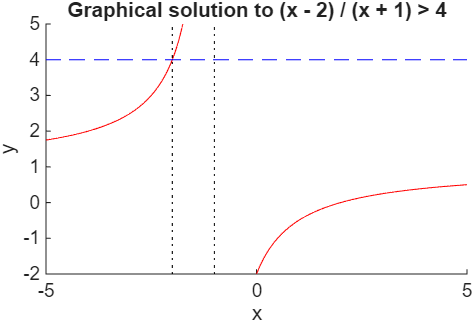
\includegraphics{images/matlab-inequalities-plot-output}
        \caption{The output of \cref{cde:matlab inequalities plot}.}
        \label{fig:inequalities example 2 matlab}
    \end{figure}
    
    \begin{exm}{}{}
        Find the set of all \(x \in \reals\) satisfying
        \begin{equation}
            \abs{3x + 6} + x < 4.
        \end{equation}
        We consider cases, \(3x + 6 \ge 0\) and \(3x + 6 < 0\):
        \begin{enumerate}
            \item If \(3x + 6 \ge 0\) then \(\abs{3x + 6} = 3x + 6\), and so we have
            \begin{equation}
                3x + 6 + x < 4
            \end{equation}
            which we can solve to find
            \begin{equation}
                x < -\frac{1}{2}.
            \end{equation}
            As a set, \(x \in (-\infty, -1/2)\).
            \item If \(3x + 6 < 0\) then \(\abs{3x + 6} = -(3x + 6)\), and so we have
            \begin{equation}
                -3x - 6 + x < 4
            \end{equation}
            which we can solve (remembering to flip the inequality when we divide by a negative) to find
            \begin{equation}
                x > -1/2
            \end{equation}
            As a set, \(x \in (-1/2, \infty)\).
        \end{enumerate}
        The solution set is then \((-\infty, -5) \cap (-1/2, \infty) = (-5, -1/2)\), so \(-5 < x < -1/2\).
    \end{exm}
    
    \begin{cde}{}{cde:mathematica inequalities plot}
        Here's some code plotting \(y = \abs{3x + 6} + x\) and \(y = 4\) in Mathematica.
        Here I use \lstinline[language=Mathematica]|Solve| to find the intersection points, then plot the graph with \lstinline[language=Mathematica]|Plot| and plot the vertical lines with \lstinline[language=Mathematica]|Line|.
        The \lstinline[language=Mathematica]|Show| and \lstinline[language=Mathematica]|Graphics| commands just make everything appear on the same plot.
        The output is \cref{fig:mathematica inequalities plot}.
        
        \begin{lstlisting}[gobble=12, language=Mathematica]
            intersectx = x /. Solve[Abs[3 x + 6] + x == 4];
            Show[{
                Plot[{Abs[3 x + 6] + x, 4}, {x, -10, 2}],
                Graphics[{Dashed, 
                    Line[{{intersectx[[1]], -2},
                        {intersectx[[1]], 14}}], 
                    Line[{{intersectx[[2]], -2},
                        {intersectx[[2]], 14}}]}]
            }]
        \end{lstlisting}
    \end{cde}
    
    \begin{figure}
        \centering
        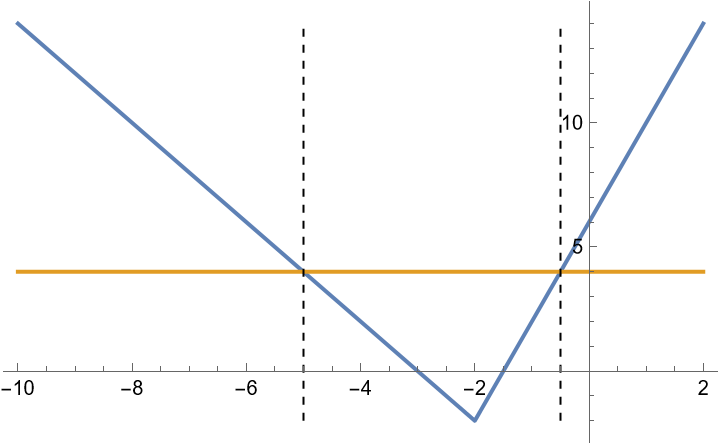
\includegraphics[width=0.8\textwidth]{images/inequalities-plot-abs-value-mathematica-output}
        \caption{The output of \cref{cde:mathematica inequalities plot}}
        \label{fig:mathematica inequalities plot}
    \end{figure}
    
    \section{Quadratics}
    A \defineindex{quadratic equation} is an equation of the form
    \begin{equation}
        \label{eqn:quardatic}
        ax^2 + bx + c = 0.
    \end{equation}
    Here \(x\) is a variable and the coefficients, \(a\), \(b\), and \(c\) are some sort of numbers.
    We'll assume our coefficients are real numbers, but sometimes it makes sense to restrict to integers, and in the next block you'll see that often it's useful to extend to complex numbers.
    
    The goal is to find all values of \(x\) which make this equation true.
    If we restrict \(x\) to be a real number then it turns out that such an equation has either \(0\), \(1\), or \(2\) solutions.
    This follows from the quadratic equation, which is our first method for solving quadratics.
    
    \subsection{Quadratic Formula}
    The \defineindex{quadratic formula} provides the solution(s), \(x\), to the quadratic equation of \cref{eqn:quardatic}.
    The solution(s) are
    \begin{equation}
        x = \frac{-b \pm \sqrt{b^2 - 4ac}}{2a}.
    \end{equation}
    
    Notice the square root.
    If \(x\) is to be a real number we can only take square roots of non-negative quantities.
    We call \(\Delta = b^2 - 4ac\) the \defineindex{discriminant} of the quadratic.
    It helps us tell the difference between which case we're in, \(0\), \(1\) or \(2\) solutions:
    \begin{itemize}
        \item If \(\Delta > 0\) then \(x = (-b + \sqrt{\Delta})/2a\) and \(x = (-b - \sqrt{\Delta})/2a\) are two distinct real solutions.
        \item If \(\Delta = 0\) then \(x = -b/2a\) is the only solution, you'll also hear this being called a repeated root (root just being another word for the solution to an equation).
        It's as if this solution somehow appears twice, we'll see why in the next section on factorisation.
        \item If \(\Delta < 0\) then we can't take the square root, and so there are no real solutions.
        You'll see in the next block that there are \emph{complex} solutions still.
        In fact, if we allow complex roots then there are always two solutions, so long as we count the repeated solutions of the \(\Delta = 0\) case as two solutions (which is why we say 2 \emph{distinct} solutions for \(\Delta > 0\)).
    \end{itemize}
    
    \begin{exm}{}{}
        Solve
        \begin{equation}
            3x^2 + x - 2 = 0
        \end{equation}
        using the quadratic equation.
        
        We simply identify \(a = 3\), \(b = 1\), and \(c = -2\).
        We then have \(\Delta = b^2 - 4ac = 1^2 - 4 \cdot 3 \cdot (-2) = 25\), which is positive, so we expect two distinct solutions.
        Plugging these values into the equation we find the solutions are
        \begin{equation}
            x = \frac{-1 \pm \sqrt{25}}{2 \cdot 3}
        \end{equation}
        which gives the solutions
        \begin{equation}
            x = \frac{-1 - 5}{6} = -1, \qqand x = \frac{-1 + 5}{6} = \frac{2}{3}.
        \end{equation}
    \end{exm}
    
    \subsection{Factorising}
    When the roots of a quadratic aren't too horrible it is often possible to factorise it.
    Then the roots are simply the values of \(x\) which make each term in the factorisation vanish.
    
    \begin{exm}{}{}
        Solve
        \begin{equation}
            3x^2 + x - 2 = 0
        \end{equation}
        by factorising.
        
        The factorisation process is a bit of an art.
        We'll assume that there are no fractions appearing as coefficients of \(x\) in the formula (you can always multiply by any denominator that appears to get rid of it).
        Then the factorisation must be of the form
        \begin{equation}
            (3x + \alpha)(x + \beta) = 0
        \end{equation}
        for some \(\alpha, \beta \in \reals\).
        There are several methods for finding \(\alpha\) and \(\beta\).
        One is just to stare at this for a while until you can see the solution.
        Another is to expand these brackets and equate coefficients, so let's do that.
        Expanding the brackets we get
        \begin{equation}
            3x^2 + \alpha x + 3\beta x + \alpha \beta = 3x^2 + (\alpha + 3\beta) x + \alpha \beta.
        \end{equation}
        Equating coefficients we have that \(\alpha + 3\beta = 1\) and \(\alpha \beta = -2\).
        These are simultaneous equations, which can also be solved in many ways.
        The second equation tells us that \(\beta = -2/\alpha\), which we can substitute into the first, giving
        \begin{equation}
            \alpha - \frac{2}{3}\alpha = 1 \implies \frac{1}{3}\alpha = 1 \implies \alpha = 3.
        \end{equation}
        Then we have \(\beta = -2/3\).
        This gives
        \begin{equation}
            \left( 3x + 3 \right)\left( x - \frac{2}{3} \right) = 0.
        \end{equation}
        For this to be true it must be that either
        \begin{equation}
            3x + 3 = 0, \qqor x - \frac{2}{3} = 0.
        \end{equation}
        Solving these equations we have
        \begin{equation}
            x = -1, \qqor x = \frac{2}{3}.
        \end{equation}
    \end{exm}
    
    Consider the quadratic \(x^2 - 2x + 1\).
    This has \(\Delta = (-2)^2 - 4 \cdot 1 \cdot 1 = 0\) and factorises as \((x - 1)^2\).
    The two factors of \(x - 1\) are why we call \(x = 1\) a repeated root of this quadratic.
    
    \subsection{Completing The Square}
    The quadratic
    \begin{equation}
        ax^2 + bx + c = 0
    \end{equation}
    can always be written as
    \begin{equation}
        a\left( x + \frac{b}{2a} \right)^2 - \frac{b^2}{4a} + c = ax^2 + bx + c,
    \end{equation}
    which you can check by expanding the left hand side.
    The process of doing so is called \defineindex{completing the square}.
    
    I advise that you \emph{don't} memorise this formula.
    Instead just practice with specific quadratics and you'll learn the process for completing the square.
    
    While completing the square is usually not the fastest way to solve a quadratic equation it can be useful if you're trying to plot a quadratic, since it's generally easier to plot a quadratic of the form \((x - p)^2 + q = 0\), since the turning point of this quadratic has a turning point at \((p, q)\).
    Be careful about signs when you do this.
    
    \begin{exm}{}{}
        Solve
        \begin{equation}
            3x^2 + x - 2 = 0
        \end{equation}
        by completing the square.
        
        First factorise out the coefficient of \(x^2\) from the \(x^2\) and \(x\) terms, giving
        \begin{equation}
            3(x^2 + x/3) - 2 = 0.
        \end{equation}
        Our goal is to write \(x^2 + x/3\) in the form \((x + p)^2 + q\) for some \(p\) and \(q\).
        To do this I like to equate coefficients, expanding we have
        \begin{equation}
            (x + p)^2 + q = x^2 + 2px + p^2 + q = x^2 + \frac{1}{3}x.
        \end{equation}
        Equating coefficients we have \(2p = 1/3\), so \(p = 1/6\).
        We also have \(p^2 + q = 0\), so \(q = -1/36\).
        Then we have
        \begin{equation}
            3\left( \left( x + \frac{1}{6} \right)^2 - \frac{1}{36} \right) - 2 = 0.
        \end{equation}
        Expanding the outer brackets this becomes
        \begin{equation}
            3\left( x + \frac{1}{6} \right)^2 - \frac{25}{12} = 0.
        \end{equation}
        At this point it's a good idea to expand fully and check that you get \(3x^2 + x - 2\) back.
        
        Now that we have this form we can add \(25/12\) to both sides, giving
        \begin{equation}
            3\left( x + \frac{1}{6} \right)^2 = \frac{25}{12}.
        \end{equation}
        Dividing by \(3\) we get
        \begin{equation}
            \left( x + \frac{1}{6} \right)^2 = \frac{25}{36}.
        \end{equation}
        To undo the squaring we take the square root, and we take \(\pm\) as well, giving
        \begin{equation}
            x + \frac{1}{6} = \pm \frac{5}{6}.
        \end{equation}
        Finally, we can add \(1/6\) to both sides giving the solution
        \begin{equation}
            x = \frac{1}{6} \pm \frac{5}{6},
        \end{equation}
        which gives the solutions
        \begin{equation}
            x = \frac{1}{6} - \frac{5}{6} = -\frac{2}{3}, \qqor x = \frac{1}{6} + \frac{5}{6} = 1.
        \end{equation}
    \end{exm}
    
    We can follow the same process as above but working with general \(a\), \(b\), and \(c\).
    Starting with 
    \begin{equation}
        a\left( x + \frac{b}{2a} \right)^2 - \frac{b^2}{4a} + c = ax^2 + bx + c,
    \end{equation}
    we can add the constant term to each side,
    \begin{equation}
        a\left( x + \frac{b}{2a} \right)^2 = \frac{b^2}{4a} - c.
    \end{equation}
    Dividing by \(a\) we get
    \begin{equation}
        \left( x + \frac{b}{2a} \right)^2 = \frac{b^2}{4a^2} - \frac{c}{a}.
    \end{equation}
    We can undo the squaring by taking square roots, remembering to include \(\pm\) so we don't lose solutions:
    \begin{equation}
        x + \frac{b}{2a} = \pm \sqrt{\frac{b^2}{4a^2} - \frac{c}{a}}.
    \end{equation}
    Some manipulation of fractions and square roots gives us
    \begin{equation}
        \sqrt{\frac{b^2}{4a^2} - \frac{c}{a}} = \sqrt{\frac{b^2 - 4ac}{4a^2}} = \frac{\sqrt{b^2 - 4ac}}{2a}.
    \end{equation}
    Finally, adding \(b/2a\) to both sides we end up with
    \begin{equation}
        x = \frac{-b \pm \sqrt{b^2 - 4ac}}{2a},
    \end{equation}
    which is exactly the quadratic equation!
    
    \subsection{Graphical Solution}
    If you can plot the quadratic then the solution is just where it crosses the \(x\)-axis.
    \Cref{fig:desmos parabola} shows a plot done in \href{https://www.desmos.com/calculator}{Desmos}.
    When you have this plot you can just hover the mouse over the line to find \emph{approximate} values.
    This isn't a great method for finding solutions with one hundred percent certainty, but you can use it to guess solutions, \(\alpha\) and \(\beta\), then plug these into \((x - \alpha)(x - \beta)\) and expand, if you guessed correctly then you'll get the original quadratic back.
    
    \begin{figure}
        \centering
        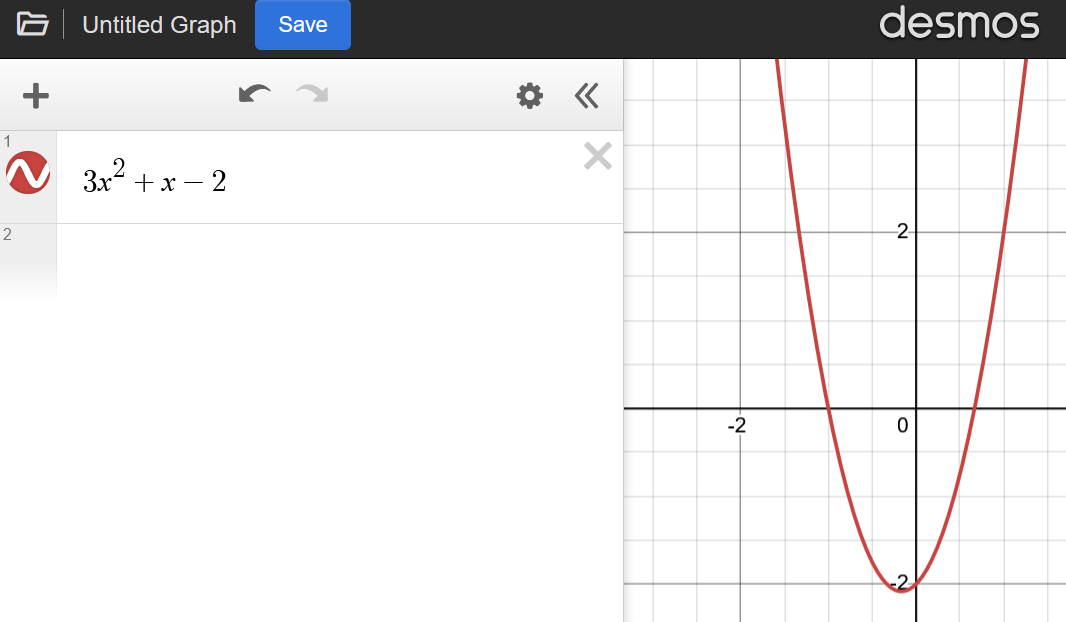
\includegraphics[width=0.8\textwidth]{images/desmos-quadratic-plot}
        \caption{Plot of \(y = 3x^2 + x - 2\) in Desmos.}
        \label{fig:desmos parabola}
    \end{figure}
    
    \subsection{Computer Solution}
    The truth is that most people aren't solving quadratics manually.
    That being said it's important to understand quadratics as the second simplest (after a straight line) case of a polynomial.
    It's also a good way to learn about roots, turning points, and other properties of more general equations.
    This means that I can't, in good conscience, suggest that you just use a computer to solve all quadratics, but it can be done, and once you've had enough practice solving quadratics by hand it's a reasonable thing to do.
    
    Note that a computer doesn't know if the solutions need to be real, so most will give you complex roots, which you can then choose to keep or exclude.
    If your solutions contain things like square roots of a negative, or the symbols \(i\) or \(j\) then that's a sign that the returned solution is complex.
    
    \begin{cde}{}{}
        Here's how to solve a quadratic equation in Matlab.
        This needs the \enquote{Symbolic Math Toolbox} add-on.
        \begin{lstlisting}[gobble=12, language=Matlab]
            syms x;
            solve(3*x^2 + x - 2 == 0)
            >>> [-1, 2/3]
        \end{lstlisting}
        
        Here's how to solve a quadratic equation in Mathematica.
        \begin{lstlisting}[gobble=12, language=Mathematica]
             In[1] Solve[3x^2 + x - 2 == 0]
            Out[1] {{x -> -1}, {x -> 2/3}}
        \end{lstlisting}
        
        Here's how to solve a quadratic equation in Python.
        This needs the \enquote{Sympy} package.
        \begin{lstlisting}[gobble=12, language=python]
            from sympy import solveset
            from sympy.abc import x
            solveset(3*x**2 + x - 2)
            >>> {-1, 2/3}
        \end{lstlisting}
    \end{cde}
    
    \subsection{Quadratic Inequalities}
    \begin{exm}{}{}
        Solve
        \begin{equation}
            3x^2 + x - 2 \le 0.
        \end{equation}
        We already know that the two key points are \(x = -2/3\) and \(x = 1\).
        It just remains to see if the inequality is satisfied between these points our outside of them.
        Looking at \cref{fig:desmos parabola} we see that the graph dips below the \(x\)-axis, which is \(y = 0\), between these points.
        So, we want between these points.
        Notice also that at these points \(3x^2 + x - 2\) is \(0\), and we want to include \(0\) since we have \(\le\).
        Therefore, the solution set is the interval \([-2/3, 1]\).
    \end{exm}
    
    \chapter{Binomial Theorem}
    \section{Index Notation}
    Suppose you're designing a part for a car engine.
    One thing you may worry about is if the part can stand up to the temperatures in a car.
    You could start the car, wait a bit, then measure the temperature of the car.
    However, this isn't a great experiment, the car is likely to be a different temperature depending on how long its been running, how hard the engine is being pushed, the external temperature, and many other factors.
    A better experiment is to add a temperature logger to the car's engine which takes a temperature measurement, say every 5 minutes.
    
    The nice thing about maths is that we can do some analysis of this data before we've even collected it!
    All we have to do is come up with a name for the data, then we can do maths with it without having to know the actual value!
    So, before you do this hypothetical experiment you might decide to give a name to every temperature you measure.
    A sensible choice is \(T\) for temperature for the first measurement.
    Then the second measurement can be \(t\).
    We can swap to Greek letters, calling the result of the next three measurements \(\tau\), \(\theta\) and \(\Theta\).
    Now we have a problem, because we've run out of T-like letters, and soon we'll run out of all letters if we keep up like this.
    If we were taking hundreds of measurements this is a really bad way to label the results.
    
    A much better idea is to call the first measurement \(T_0\), then the second \(T_1\) and the third \(T_2\) and so on.
    We've chosen to start at \(0\), but you can start at \(1\) as well, you just have to adjust other things later.
    Similarly, we might label the times at which the measurements were made \(t_0\), \(t_1\), and so on.
    For short, we call our measurements \(T_i\) and \(t_i\), where \(i\) is standing in for any \defineindex{index} (that's what we call the subscript letter), which usually means \(i = 1, \dotsc, N\), where \(N + 1\) is the total number of measurements we take.
    
    One important value to consider in our experiment is the maximum temperature, which we might denote \(\max\{T_i\}\).
    Another value that might be important, say if we're worried about thermal expansion, is the rate of temperature change.
    We can approximate the rate of temperature change between times \(t_i\) and \(t_{i+1}\) as
    \begin{equation}
        \frac{T_{i+1} - T_i}{t_{i+1} - t_i}.
    \end{equation}
    Note that \(t_{i+1} - t_i\) is just 5 minutes, so \((T_{i+1} - T_i)/5\) will give us the temperature change in degrees per minute (assuming \(T_i\) is measured in degrees celsius).
    
    Another important value is the average temperature, which can be computed as
    \begin{equation}
        \frac{T_0 + T_1 + \dotsb + T_N}{N + 1}.
    \end{equation}
    This \(\dotsb\) is sometimes not quite as precise as we need.
    Instead, we have a special notation for sums like this.
    
    \begin{ntn}{Sigma Notation}{}
        If \(T_0, \dotsc, T_N\) are some values then we write
        \begin{equation}
            \label{eqn:sum}
            \sum_{k=0}^N T_k
        \end{equation}
        for
        \begin{equation}
            T_0 + T_1 + \dotsb + T_N.
        \end{equation}
    \end{ntn}
    
    \begin{remark}{}{}
        The \(\sum\) symbol comes from the Greek letter \(\Sigma\) (sigma), which is just a capital S for Sum.
    \end{remark}
    
    We read \cref{eqn:sum} as \enquote{the sum from \(k = 0\) to \(N\) of \(T_k\)}.
    We call \(k = 0\) and \(N\) the \define{limits}\index{limit!of sum} of the sum.
    To evaluate the expression\footnote{Note that inline it's common to move the limits of the sum up and to the side.} \(\sum_{k=0}^N T_k\) we start with \(k = 0\), which gives us \(T_0\), then \(k = 1\), which gives \(T_1\), and so on, up to \(k = N\), which gives \(T_N\).
    We sum up these results, giving \(T_0 + T_1 + \dotsb + T_N\).
    
    \begin{exm}{}{}
        \begin{itemize}
            \item \(\displaystyle\sum_{k=0}^5 T_k = T_0 + T_1 + T_2 + T_3 + T_4 + T_5\);
            \item \(\displaystyle\sum_{r=2}^7 r^2 = 2^2 + 3^2 + 4^2 + 6^2 + 7^2 = 114\);
            \item \(\displaystyle\sum_{\ell=-5}^{-2} \ell(\ell + 1) = -5(-5 + 1) + -4(-4 + 1) + -3(-3 + 1) + -2(-2 + 1) = 40\);
            \item \(\displaystyle\sum_{i=4}^6 \frac{2}{i}\alpha_i = \frac{2}{4}\alpha_4 + \frac{2}{5} \alpha_5 + \frac{2}{6} \alpha_6 = \frac{1}{2} \alpha_4 + \frac{2}{5}\alpha_5 + \frac{1}{3} \alpha_6\).
            \item \(\displaystyle\sum_{i=1}^3 \sum_{j=1}^3 a_i b_j\), first evaluate the inner sum, \(\sum_{j=1}^3 b_j = b_1 + b_2 + b_3\), and then the outer one, giving
            \begin{equation}
                a_1(b_1 + b_2 + b_3) + a_2(b_1 + b_2 + b_3) + a_3(b_1 + b_2 + b_3).
            \end{equation}
            Of course, you can expand this, and rearrange the terms to write it in different ways.
        \end{itemize}
    \end{exm}
    
    \begin{problem}{}{}
        Evaluate the following sums\footnote{Ans: 362, 6, 3025, 175}
        \begin{itemize}
            \item \(\displaystyle\sum_{x=7}^{10} (x^2 + 2x)\);
            \item \(\displaystyle\sum_{\alpha = -2}^{2} \abs{\alpha}\);
            \item \(\displaystyle\sum_{s=1}^{10} s^3\);
            \item \(\displaystyle\sum_{i=1}^7 \sum_{j=1}^2 (2i + 3j)\)
        \end{itemize}
    \end{problem}
    
    \begin{wrn}
        Sometimes you'll see sums where one of the limits is \(\infty\).
        You have to be careful with these sums because sometimes it doesn't make sense to sum together infinitely many things.
    \end{wrn}
    
    \begin{wrn}
        Note that \(i\) and \(j\) are both commonly used as indices in sums.
        Don't confuse them with the complex unit, \(\sqrt{-1}\).
    \end{wrn}
    
    \begin{remark}{}{}
        When you have to write lots of sums writing \(k = 0\) and \(N\) over and over gets pretty tiresome.
        You'll probably see people write
        \begin{equation}
            \displaystyle \sum_{k} T_k \qqor \sum T_k.
        \end{equation}
        You then have to work out where \(k\) starts and finishes from context, or even that it's \(k\) that is being summed in the first place!
        Avoid doing this until you are really comfortable with the sum notation, and avoid doing it in exams as well.
    \end{remark}
    
    Using this notation we can write the average temperature as
    \begin{equation}
        \frac{1}{N + 1} \sum_{k = 0}^{N} T_k.
    \end{equation}
    
    This notation is very useful, and very common, so make sure you're happy with it.
    There's a similar notation for multiplication.
    
    \begin{ntn}{}{}
        If \(T_0, \dotsc, T_N\) are some values we write
        \begin{equation}
            \prod_{k=0}^N T_k
        \end{equation}
        for
        \begin{equation}
            T_0 T_1 \dotsm T_N.
        \end{equation}
    \end{ntn}
    
    \begin{remark}{}{}
        The \(\prod\) symbol comes from the Greek letter \(\Pi\) (pi) which is just capital P for product.
    \end{remark}
    
    \section{Factorials and Binomial Coefficients}
    \begin{dfn}{Factorial}{}
        For \(n \in \naturals\) we define the \defineindex{factorial} of \(n\), written \(n!\) and read \enquote{\(n\) factorial}, to be the product of all of the whole numbers from \(1\) to \(n\).
        That is,
        \begin{equation}
            n! = 1 \cdot 2 \cdot \dotsb (n - 1) n.
        \end{equation}
    \end{dfn}
    
    \begin{exm}{}{}
        Here's \(n!\) for \(n = 1, \dotsc, 10\):
        \begin{equation*}
            \begin{array}{r|rrrrrrrrrr}
                n & 1 & 2 & 3 & 4 & 5 & 6 & 7 & 8 & 9 & 10 \\ \hline
                n! & 1 & 2 & 6 & 24 & 120 & 720 & 5040 & 40320 & 362880 & 3628800
            \end{array}
        \end{equation*}
        Notice how quickly the factorial grows, by \(10\) we're already at about 3.6 million! [That's an exclamation mark, not another factorial]
    \end{exm}
    
    If you start calculating some factorials by hand you'll realise that you're doing the same calculations over and over.
    For example, if we compute \(6!\) we need to compute \(5!\) along the way:
    \begin{equation}
        6! = \underbrace{1 \cdot 2 \cdot 3 \cdot 4 \cdot 5}_{5!} \cdot 6.
    \end{equation}
    In general, if we compute \(n!\) we need to compute \((n-1)!\) along the way:
    \begin{equation}
        n! = \underbrace{1 \dotsm (n - 1)}_{(n-1)!} n.
    \end{equation}
    This gives us a recursive way to compute factorials, which can also be taken as an alternative definition.
    For \(n \in \naturals\) we have
    \begin{equation}
        n! \coloneq 
        \begin{cases}
            1 & n = 1;\\
            (n - 1)! \cdot n & n > 1.
        \end{cases}
    \end{equation}
    
    \begin{cde}{}{}
        Here's a python program which computes the factorial of an input:
        \begin{lstlisting}[gobble=12, language=python]
            def factorial(n: int) -> int:
                if n == 1:
                    return 1
                return n * factorial(n - 1)
        \end{lstlisting}
        Note that this is \emph{not} an efficient way to compute this, but it's the most direct implementation of the equation above.
        Also, better code would check for invalid inputs, such as negative numbers, or non-integers, but that gets in the way of understanding the maths.
        
        Here's a similar implementation in Haskell
        \begin{lstlisting}[language=haskell, gobble=12]
            factorial :: Int -> Int
            factorial 1 = 1
            factorial n = n * factorial (n - 1)
        \end{lstlisting}
        The first line just says the input and output are both integers.
        Haskell can automatically determine cases from this list of definitions.
    \end{cde}
    
    One sensible question after we define something is \enquote{so what}?
    Why should we care about the factorial?
    One answer is that \(n!\) is the number of ways to arrange \(n\) (distinct) objects in a row.
    If we have the set \(\{1, 2\}\) there are \(2\) different ways to order these elements, \enquote{\(12\)} or \enquote{\(21\)}.
    If we have the set \(\{1, 2, 3\}\) there are \(6\) different ways to order these elements, \enquote{\(123\)}, \enquote{\(132\)}, \enquote{\(213\)}, \enquote{\(231\)}, \enquote{\(312\)} or \enquote{\(321\)}.
    We can keep going like this, there are \(24\) different ways to order the elements of \(\{1, 2, 3, 4\}\), and so on.
    
    Notice that we can rearrange the second part of the recursive definition to get that \((n-1)! = n!/n\).
    Using this we can extend the definition of factorial to \(0\).
    If \(n - 1 = 0\) then \(n = 1\) and we have
    \begin{equation}
        0! = \frac{1!}{1} = \frac{1}{1} = 1.
    \end{equation}
    We then extend our definition of factorial to all non-negative integers by defining \(0! \coloneq 1\).
    
    \begin{remark}{}{}
        There are several other justifications for why \(0! = 1\) is the correct definition to make.
        At the end of the day we make definitions in maths because they're useful, and \(0! = 1\) is the most useful definition, mostly because it fits into lots of patterns, including the following.
        
        \begin{itemize}
            \item Think about \(n!\) as the number of ways of arranging \(n\) things.
            If we have \(\{1\}\) then there's only one way to order the elements, \enquote{\(1\)}.
            If we have \(\emptyset = \{\}\) then there's also only one way to order the elements, \enquote{\(\)} (that's the empty list, but it's still a valid ordering of no things).
        
            \item Next year you'll learn some \href{https://en.wikipedia.org/wiki/Complex_analysis}{complex analysis}, in that course you may come across the \href{https://en.wikipedia.org/wiki/Gamma_function}{gamma function},
            \begin{equation}
                \Gamma(z) \coloneq \int_0^{\infty} t^{z - 1} \e^{-t} \dd{t}.
            \end{equation}
            Don't worry about any of these symbols if they're not familiar or just a bit scary.
            The important thing is that you can show that the gamma function is such that \(\Gamma(n) = (n - 1)!\) for any \(n \in \naturals\), and also \(\Gamma(1) = 1\) so we should define \((1 - 1)! = 0! = 1\) if we want this pattern to continue.
            The gamma function actually allows us to extend the factorial to negative numbers and even non-whole numbers!
            For example, you can evaluate this function at \(3/2\) and you find that \(\Gamma(3/2) = \sqrt{\pi}\).
            If you spend enough time in proximity to \enquote{Popular Maths}, say on Youtube, you'll probably see someone claiming that \(1/2\) factorial is \(\sqrt{\pi}\), and this is what they mean.
            It isn't really correct to call this the factorial though unless the input is a positive whole number (which then includes \(0! = \Gamma(1)\) since \(1\) is positive).
        \end{itemize}
     \end{remark}
     
     A reasonable question, following on from the question of ordering things, is the following.
     If I have a set of \(n\) objects how many different ways can I pick \(k\) of them?
     When faced with a question like this it's often good to look at a few examples with small numbers.
     If \(k = 0\) then there's one way to pick a set of \(0\) elements from \(\{1, \dotsc, n\}\), you take \(\emptyset\).
     Similarly, if \(k = n\) then there's only one way to pick a set of \(n\) elements from \(\{1, \dotsc, n\}\), you take \(\{1, \dotsc, n\}\).
     If \(k = 1\) then there's \(n\) ways to pick a set of \(1\) element from \(\{1, \dotsc, n\}\), we could take \(\{1\}\), \(\{2\}\), and so on up to \(\{n\}\).
     
     If \(k = 2\) then things are a bit trickier, so let's fix a value of \(n\) as well, say \(n = 4\).
     We can take \(\{1, 2\}\), \(\{1, 3\}\), \(\{1, 4\}\), \(\{2, 3\}\), \(\{2, 4\}\), or \(\{3, 4\}\).
     That's \(6\) different ways to make the choice.
     If you keep playing around with small values, and if you pick the sets in a sensible order, then you may start to see a pattern emerging.
     The key is to think about ordering the items, and then forgetting the orders again at the end.
     We've been doing this implicitly by choosing to call our elements \(1, \dotsc, n\).
     
     Here's a way to pick \(k\) elements from any \(n\) element set.
     First, order the \(n\) elements in some way.
     There are \(n!\) ways to do this.
     Then pick the first \(k\) elements.
     There's a problem with this though, if I swap two elements amongst the first \(k\) the result doesn't change, and if I swap two elements among the last \(n - k\) the result doesn't change again.
     For example, if \(n = 6\) and \(k = 3\) then I can order my elements as \(123456\).
     Then I take the first three elements, \(123\).
     Forgetting the order this gives us the set \(\{1, 2, 3\}\).
     However, if I'd picked any of the orders \(132456\), \(123465\), \(132465\), and so on I would still result in picking \(\{1, 2, 3\}\) as the final set (although the order may be different, but that's not important for a set).
     
     What we see is that the \(n!\) ways to order these elements results in us over counting the number of subsets of size \(k\).
     In particular, we over count by a factor of the number of ways of rearranging the first \(k\) elements, which is \(k!\), and a factor of the number of ways of arranging the last \(n - k\) elements, which is \((n - k)!\).
     The result is that the number of ways of picking \(k\) things from a set of \(n\) things is
     \begin{equation}
         \frac{n!}{k!(n - k)!}.
     \end{equation}
     
     \begin{dfn}{Binomial Coefficient}{}
         The \defineindex{binomial coefficient} is defined by
         \begin{equation}
             \binom{n}{k} = {}_nC_k = {}^nC_k \coloneq \frac{n!}{k!(n - k)!}.
         \end{equation}
     \end{dfn}
     
     The reason for the name \enquote{binomial coefficient} will become clear in the next section.
     
     \begin{problem}{}{}
         Compute the following binomial coefficients\footnote{Ans: 10, 6, 10, 20, 252}.
         For the first three try using the formula and counting the number of subsets.
         For the others you can just use the formula
         \begin{equation}
             \binom{5}{3}; \quad \binom{6}{3}; \quad \binom{4}{2}; \quad \binom{10}{9}; \qand \binom{10}{5}.
         \end{equation}
         Hint: Finding subsets with \(9\) out of \(10\) things is the same as finding subsets which don't contain \(1\) out of \(10\) things.
     \end{problem}
     
     \subsection{Binomial Expansion}
     A \defineindex{binomial} is any expression of the form \(a + b\).
     The expansion part is that we often need to compute \((a + b)^2\), \((a + b)^3\), or even higher powers.
     Fortunately, there's a fast way to do it.
     We can use the \defineindex{binomial theorem}.
     
     \begin{thm}{Binomial Theorem}{}
         For \(n \in \naturals\) we have
         \begin{equation}
             (a + b)^n = \sum_{k=0}^n \binom{n}{k} a^{n-k}b^k.
         \end{equation}
     \end{thm}
     
     \begin{exm}{}{}
         Compute \((x + 3)^2\):
         \begin{align}
             (x + 3)^2 &= \sum_{k=0}^2 \binom{2}{k} x^{2 - k}3^k\\
             &= \binom{2}{0} x^{2 - 0} 3^0 + \binom{2}{1} x^{2 - 1} 3^1 + \binom{2}{2} x^{2 - 2} 3^2\\
             &= x^2 + 2 x \cdot 3 + 9\\
             &= x^2 + 6x + 9.
         \end{align}
         
         Compute \((a + b)^3\):
         \begin{align}
             (a + b)^3 &= \sum_{k=0}^3 \binom{3}{k} a^{3 - k} b^k\\
             &= \binom{3}{0} a^{3 - 0} b^0 + \binom{3}{1} a^{3 - 1} b^1 + \binom{3}{2} a^{3 - 2} b^2 + \binom{3}{3} a^{3 - 3} b^3\\
             &= a^3 + 3a^2b + 3ab^2 + b^3.
         \end{align}
         
         Compute \((x + y)^4\):
         \begingroup
         \allowdisplaybreaks
         \begin{align}
             (a + b)^4 &= \sum_{k=0}^4 \binom{4}{k} x^{4 - k} y^k\\
             &= \binom{4}{0} x^4 y^0 + \binom{4}{1} x^3 y^1 + \binom{4}{2} x^2 y^2 + \binom{4}{3} x^1 y^3 + \binom{4}{4} x^0 y^4\\
             &= x^4 + 4x^3y + 6x^2y^2 + 4xy^3 + y^4.
         \end{align}
         \endgroup
     \end{exm}
     
     Some things to notice which help you avoid errors:
     \begin{itemize}
         \item If you add up the exponents (including 1) in each term you'll always get \(n\).
         In the last example we get \(4 + 0\), \(3 + 1\), \(2 + 2\), \(1 + 3\), and \(0 + 4\), all of which add up to \(4\).
         \item The coefficients should increase up to some value, then decrease in reverse.
         For these three examples the coefficients go \(1, 2, 1\), then \(1, 3, 3, 1\), then \(1, 4, 6, 4, 1\).
     \end{itemize}
     
     The nice thing about the binomial theorem (also known as the binomial formula) is that you don't always have to compute the whole thing.
     Suppose you just want to know what the coefficient of \(h^{32}\) is in \((x/y + h)^{50}\).
     You can compute this, it's just
     \begin{equation}
         \binom{50}{32} \left( \frac{x}{y} \right)^{50 - 32} = 18053528883775\frac{x^{18}}{y^{18}}.
     \end{equation}
     Okay, that's a bit of a silly example, but it really is useful to be able to quickly determine coefficients of single terms sometimes.
     
     \begin{exm}{}{}
         Suppose you're computing interest.
         If the interest is paid at a rate of \(5\%\) annually then after \(3\) years the amount is \(1.05^3N\) where \(N\) is the original amount.
         If you don't have a calculator you can compute \(1.05^n\) using the binomial expansion.
         First, write \(1.05 = 1 + 0.05\) and note that \(0.05 = 5/100\).
         Then we have
         \begin{align}
             1.05^3 &= \left( 1 + \frac{5}{100} \right)^3\\
             &= \sum_{k=0}^{3} \binom{3}{k} 1^{3 - k} \frac{5^k}{100^k}\\
             &= \binom{3}{0} + \binom{3}{1} \frac{5}{100} + \binom{3}{2} \frac{5^2}{100^2} + \binom{3}{3} \frac{5^3}{100^3}\\
             &= 1 + 3 \cdot \frac{5}{100} + 3 \cdot \frac{25}{10000} + \frac{125}{1000000}\\
             &= 1 + \frac{15}{100} + \frac{75}{10000} + \frac{125}{1000000}
         \end{align}
         If we only care about computing things to the nearest thousandth then we can approximate this as
         \begin{equation}
             1.05^3 \approx 1 + \frac{15}{100} = 1 + 0.15 = 1.15.
         \end{equation}
         If we want more accuracy we can include more terms.
         Including all of them gives
         \begin{equation}
             1 + 0.15 + 0.0075 + 0.000125 = 1.157625.
         \end{equation}
         All of that can be done without a calculator, and actually gave one more decimal place of accuracy than the first calculator I checked it with!
     \end{exm}
     
     \begin{remark}{}{}
         Computing approximations like this, where we are adding smaller and smaller terms, will generalise to the notion of Taylor series.
         We'll discuss these in Block 4.
     \end{remark}
     
     As you practice this you'll likely learn the coefficients for the first few exponents off by heart.
     In fact, there's a chance you recognise them already.
     Pascal's triangle (\cref{fig:pascals triangle}) is constructed by starting with \(1\)s on two sides.
     Then the rule to fill in the triangle is that each element is the sum of the two elements above it to either side.
     The result is that the rows are exactly the coefficients of the binomial expansion corresponding to that row number, that is, the binomial coefficients!
     
     \begin{figure}
         \centering
         % Code from https://tex.stackexchange.com/a/198941/180184
         % Released under CC BY-SA 3.0
         \tikzsetnextfilename{pascals-triangle}
         \tikz[x=1cm*sin 60, y=1.5cm*cos 60]
         \foreach \n in {0,...,11}
         \foreach \k in {0,...,\n}    
         \node [hexagon] at (-\n/2+\k, -\n) {\directlua{tex.print("" .. nchoosek(\n,\k))}};
         \caption{Pascal's triangle.}
         \label{fig:pascals triangle}
     \end{figure}
\end{document}